\documentclass[aspectratio=169,12pt]{beamer}

\usepackage[T1]{fontenc}
\usepackage[utf8]{inputenc}
\usepackage[default,scale=0.95]{opensans}
\usepackage{tgheros}
\usepackage[tracking=true]{microtype}
\usepackage{graphicx}
\usepackage{booktabs}
\usepackage{tabularx}
\usepackage{array}
\usepackage{amsmath}
\usepackage{tikz}
\usetikzlibrary{arrows.meta,positioning,calc,fit,backgrounds}
\usepackage{pgfplots}
\pgfplotsset{compat=1.18}

\setbeamertemplate{navigation symbols}{}
\setbeamertemplate{caption}[numbered]

% Greyscale palette following the reference deck (smth.pdf); the old colour
% names are kept so every chart and box below picks up the new style.
\definecolor{Ink}{HTML}{3F3F3F}
\definecolor{Navy}{HTML}{1F1F1F}
\definecolor{Teal}{HTML}{5A5A5A}
\definecolor{Sea}{HTML}{7A7A7A}
\definecolor{Coral}{HTML}{9A9A9A}
\definecolor{Gold}{HTML}{BDBDBD}
\definecolor{Mist}{HTML}{F2F2F2}
\definecolor{Paper}{HTML}{FFFFFF}
\definecolor{Slate}{HTML}{8A8A8A}
\definecolor{SoftRed}{HTML}{EDEDED}
\definecolor{SoftTeal}{HTML}{F2F2F2}
\definecolor{SoftGold}{HTML}{F5F5F5}
\definecolor{Rule}{HTML}{2B2B2B}

\setbeamercolor{normal text}{fg=Ink,bg=Paper}
\setbeamercolor{structure}{fg=Ink}
\setbeamercolor{frametitle}{fg=Ink,bg=Paper}
\setbeamercolor{alerted text}{fg=Navy}
\setbeamercolor{itemize item}{fg=Ink}
\setbeamercolor{enumerate item}{fg=Ink}
\setbeamertemplate{itemize item}{\small\textbullet}
\setbeamertemplate{enumerate item}{\insertenumlabel.}
\setbeamerfont{normal text}{size=\fontsize{13}{16}}

% Heavy, tightly tracked heading face for titles and section slides
\newcommand{\headfont}{\fontfamily{qhv}\fontseries{b}\selectfont}
\newcommand{\heading}[1]{{\headfont\textls[-45]{\MakeUppercase{#1}}}}

\setbeamersize{text margin left=1.05cm,text margin right=0.55cm}

% Grey gradient bar down the left edge, as in the reference deck
\setbeamertemplate{background}{%
  \begin{tikzpicture}[remember picture,overlay]
    \shade[top color=Ink,bottom color=Ink,middle color=Gold]
      ([xshift=0.62cm]current page.south west) rectangle ([xshift=0.70cm]current page.north west);
  \end{tikzpicture}%
}

\newsavebox{\titlebox}
\setbeamertemplate{frametitle}{%
  \nointerlineskip
  \vspace{0.16cm}
  \sbox\titlebox{\fontsize{22}{24}\color{Ink}\heading{\insertframetitle}}%
  \begin{beamercolorbox}[wd=\textwidth,center]{frametitle}
    \ifdim\wd\titlebox>0.96\textwidth\resizebox{0.96\textwidth}{!}{\usebox\titlebox}\else\usebox\titlebox\fi
  \end{beamercolorbox}
  \vspace{0.04cm}
  {\centering\color{Rule}\rule{0.72\textwidth}{0.45pt}\par}
  \vspace{0.02cm}
}

\setbeamertemplate{footline}{}

\newcommand{\source}[1]{\vfill}
\newcommand{\metric}[1]{\textcolor{Navy}{\bfseries #1}}
\newcommand{\caveat}[1]{\textcolor{Navy}{\bfseries\itshape #1}}
\newcommand{\softbox}[2]{%
  \begin{tikzpicture}[baseline=(n.base)]
    \node[rounded corners=2pt,fill=#1,inner xsep=5pt,inner ysep=3pt,text=Ink] (n) {#2};
  \end{tikzpicture}%
}
\newcommand{\smallstatus}[2]{\textcolor{Navy}{\bfseries #2}}

% One method entry on the Methods Overview slide
\newcommand{\methoditem}[3]{%
  {\fontsize{8.4}{10}\selectfont\textbf{#1}\hspace{0.6em}\textbf{#2}\par}
  \vspace{2pt}
  {\fontsize{7.6}{9.2}\selectfont #3\par}
  \vspace{0.24cm}
}

% Method slide: left = method, right = plot, results and lesson
\newcommand{\lesson}[1]{\colorbox{Mist}{\parbox{0.965\linewidth}{\fontsize{7.2}{8.7}\selectfont #1}}}

% Simple CLEVR-like objects for the S4 collage illustration (used inside tikzpicture)
\newcommand{\objcube}[3]{\fill[#1!80!black] (#2-0.13,#3-0.13) rectangle (#2+0.13,#3+0.13);}
\newcommand{\objball}[3]{\shade[ball color=#1] (#2,#3) circle (0.14);}
\newcommand{\objcyl}[3]{\fill[#1!80!black] (#2-0.11,#3-0.12) rectangle (#2+0.11,#3+0.10); \fill[#1!45!white] (#2,#3+0.10) ellipse (0.11 and 0.04); \fill[#1!80!black] (#2,#3-0.12) ellipse (0.11 and 0.04);}
\newcommand{\panel}[2]{\draw[Slate,fill=gray!18] (#1-0.22,#2-0.22) rectangle (#1+0.22,#2+0.22);}

% Full-slide section title
\newcommand{\sectionslide}[1]{%
  \begin{frame}[plain]
    \vfill
    \begin{center}
      {\fontsize{46}{50}\color{Ink}\heading{#1}}\par
      \vspace{0.30cm}
      {\color{Rule}\rule{0.55\textwidth}{0.45pt}}
    \end{center}
    \vfill
  \end{frame}
}

\pgfplotsset{
  deckaxis/.style={
    axis line style={draw=Slate!65},
    tick style={draw=Slate!65},
    tick label style={font=\scriptsize,color=Ink},
    label style={font=\scriptsize,color=Ink},
    title style={font=\small\bfseries,color=Ink},
    legend style={draw=none,fill=none,font=\scriptsize},
    grid=major,
    major grid style={draw=Mist},
    every node near coord/.append style={text=Ink},
  }
}

\title{What Is the Price of a Model's Eye?}
\subtitle{Understanding How VLMs Answer Multiple Choice Questions in Multimodal Settings}
\author{}
\institute{}
\date{ANLP Project \hspace{0.4em} | \hspace{0.4em} Final Presentation}

\begin{document}

% Title
\begin{frame}[plain]
  \vfill
  \begin{center}
    {\fontsize{34}{38}\color{Ink}\headfont\textls[-40]{What Is the Price of\\[2pt] a Model's Eye?}}\par
    \vspace{0.35cm}
    {\color{Rule}\rule{0.55\textwidth}{0.45pt}}\par
    \vspace{0.30cm}
    {\large\color{Ink}Understanding How VLMs Answer Multiple Choice Questions\\[2pt] in Multimodal Settings}\par
    \vspace{0.30cm}
    {\normalsize\color{Slate}ANLP Project \quad | \quad Final Presentation}
  \end{center}
  \vfill
\end{frame}

%======================================================================
\sectionslide{Introduction}

\begin{frame}{Project Idea}
\begin{columns}[T,onlytextwidth]
\column{0.56\textwidth}
\centering\small
How do mainstream vision-language models perform on formatted multiple-choice question answering tasks?

\vspace{0.32cm}
How do VLMs answer these MCQ questions, and where do those choices appear internally?

\vspace{0.32cm}
Which internal states and attention heads carry the visual answer content, map it onto an option, and write the answer symbol?
\column{0.40\textwidth}
% Space reserved for a diagram to be added later
\vspace*{3.3cm}
\end{columns}

\vspace{0.35cm}
\begin{center}\footnotesize\bfseries RESEARCH QUESTIONS\end{center}
\vspace{-0.15cm}
\begin{columns}[T,onlytextwidth]
\column{0.31\textwidth}
\centering\footnotesize
\textbf{1.} Where does visual content travel?
\column{0.31\textwidth}
\centering\footnotesize
\textbf{2.} Which components write the final symbol?
\column{0.34\textwidth}
\centering\footnotesize
\textbf{3.} Does the route survive new models, alphabets, and datasets?
\end{columns}
\end{frame}

\begin{frame}{Four models, one intervention interface}
\centering
\resizebox{0.97\textwidth}{!}{%
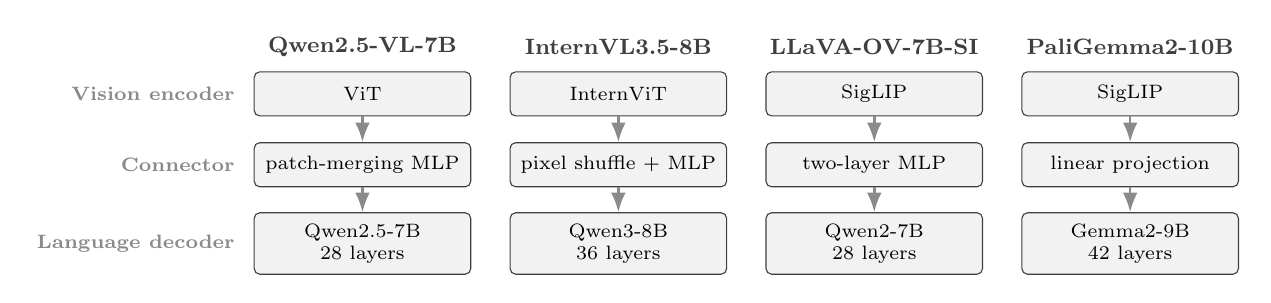
\begin{tikzpicture}[x=1cm,y=1cm,>=Latex,
  blk/.style={draw=Ink,fill=Mist,rounded corners=2pt,minimum width=2.75cm,minimum height=0.56cm,align=center,font=\scriptsize}]
\node[font=\footnotesize\bfseries,text=Ink] (nq) at (0,1.55) {Qwen2.5-VL-7B};
\node[blk] (vq) at (0,0.95) {ViT};
\node[blk] (cq) at (0,0.05) {patch-merging MLP};
\node[blk,minimum height=0.78cm] (dq) at (0,-0.95) {Qwen2.5-7B\\28 layers};
\draw[->,Slate,line width=0.9pt] (vq) -- (cq);
\draw[->,Slate,line width=0.9pt] (cq) -- (dq);
\node[font=\footnotesize\bfseries,text=Ink] (ni) at (3.25,1.55) {InternVL3.5-8B};
\node[blk] (vi) at (3.25,0.95) {InternViT};
\node[blk] (ci) at (3.25,0.05) {pixel shuffle + MLP};
\node[blk,minimum height=0.78cm] (di) at (3.25,-0.95) {Qwen3-8B\\36 layers};
\draw[->,Slate,line width=0.9pt] (vi) -- (ci);
\draw[->,Slate,line width=0.9pt] (ci) -- (di);
\node[font=\footnotesize\bfseries,text=Ink] (nl) at (6.5,1.55) {LLaVA-OV-7B-SI};
\node[blk] (vl) at (6.5,0.95) {SigLIP};
\node[blk] (cl) at (6.5,0.05) {two-layer MLP};
\node[blk,minimum height=0.78cm] (dl) at (6.5,-0.95) {Qwen2-7B\\28 layers};
\draw[->,Slate,line width=0.9pt] (vl) -- (cl);
\draw[->,Slate,line width=0.9pt] (cl) -- (dl);
\node[font=\footnotesize\bfseries,text=Ink] (np) at (9.75,1.55) {PaliGemma2-10B};
\node[blk] (vp) at (9.75,0.95) {SigLIP};
\node[blk] (cp) at (9.75,0.05) {linear projection};
\node[blk,minimum height=0.78cm] (dp) at (9.75,-0.95) {Gemma2-9B\\42 layers};
\draw[->,Slate,line width=0.9pt] (vp) -- (cp);
\draw[->,Slate,line width=0.9pt] (cp) -- (dp);
\node[anchor=east,font=\scriptsize\bfseries,text=Slate] at (-1.50,0.95) {Vision encoder};
\node[anchor=east,font=\scriptsize\bfseries,text=Slate] at (-1.50,0.05) {Connector};
\node[anchor=east,font=\scriptsize\bfseries,text=Slate] at (-1.50,-0.95) {Language decoder};
\end{tikzpicture}}

\vspace{0.30cm}
\footnotesize
After screening tests on our task, we chose the best model in each of the four families. Every model had to fit our available GPUs and expose decoder hooks for patching.

\vspace{0.14cm}
We extend the text-only analysis of \textbf{Answer, Assemble, Ace (AAA)}, so we chose models whose results can be compared with the models AAA studied.
\source{Final report Table 6 and the frozen 12-checkpoint screen}
\end{frame}

%======================================================================
\sectionslide{Dataset}

\begin{frame}{CLEVR counterfactual pairs}
\begin{columns}[T,onlytextwidth]
\column{0.52\textwidth}
\centering
\begin{minipage}[t]{0.48\linewidth}\centering
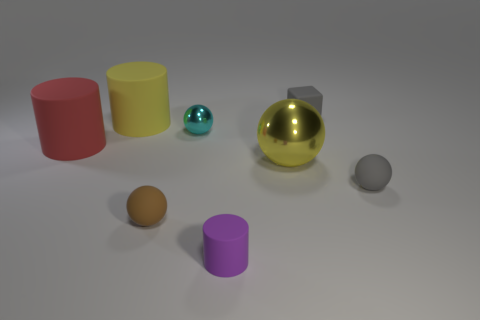
\includegraphics[width=\linewidth]{assets/clevr_pair_x.png}\\[1pt]
{\scriptsize original: sphere is yellow}
\end{minipage}\hfill
\begin{minipage}[t]{0.48\linewidth}\centering
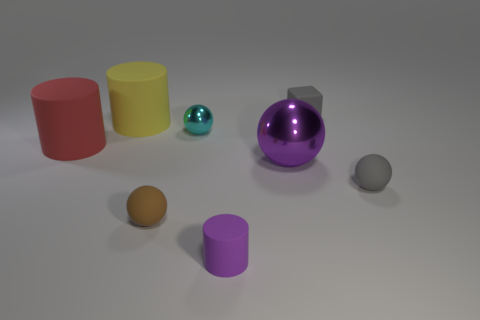
\includegraphics[width=\linewidth]{assets/clevr_pair_y.png}\\[1pt]
{\scriptsize edited: sphere is purple}
\end{minipage}

\vspace{0.14cm}
\begin{minipage}{\linewidth}\raggedright\scriptsize
What color is the large sphere that is in front of the yellow cylinder?\\[1pt]
A. yellow \quad B. gray \quad C. red \quad D. purple\\[1pt]
Respond with only the option label.\\
Answer:
\end{minipage}

\vspace{0.12cm}
{\small Correct answer: \textbf{A} (original) $\;\longrightarrow\;$ \textbf{D} (edited)}

\column{0.44\textwidth}
\centering\footnotesize
We took the \textbf{CLEVR} dataset. Each image comes with detailed scene metadata: every object's shape, colour, size, material and position.

\vspace{0.20cm}
We made a single change in that metadata and re-rendered the image. This gives a \textbf{counterfactual pair}: the same question and options, but a different correct answer.

\vspace{0.20cm}
\textbf{12 prompt variants per item}\par
\vspace{0.04cm}
4 option orders (the correct answer in each position)\\
$\times$ 3 label sets: A/B/C/D, 1/2/3/4, Q/Z/R/X
\end{columns}
\source{CLEVR-MCQ-4 v3}
\end{frame}


\begin{frame}{Types of activation patching}
\scriptsize
\renewcommand{\arraystretch}{1.0}
\begin{tabularx}{\textwidth}{@{}>{\raggedright\arraybackslash\bfseries}p{2.6cm}X>{\raggedright\arraybackslash}p{4.6cm}@{}}
\toprule
Comparison & What changes & Question it isolates \\
\midrule
Position only & Same image and answer meaning; move the correct option. & Can the model remap an option position to a new output label? \\
Content only & Edit the image so the answer meaning changes; keep its position fixed. & Does visual answer content transfer without changing the label? \\
Content + position & Change both the visual answer and its listed position. & Does the full content-to-label route transfer? \\
\bottomrule
\end{tabularx}

\vspace{0.22cm}
\centering
\textbf{Example: content + position patching}

\vspace{0.12cm}
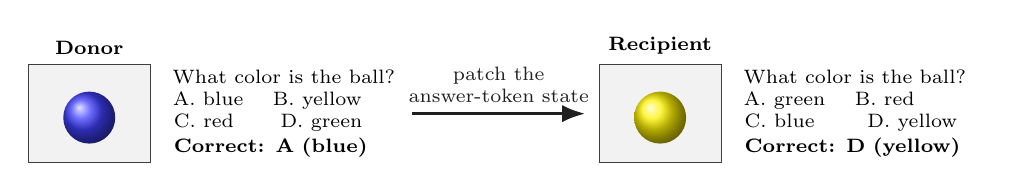
\begin{tikzpicture}[>=Latex,font=\scriptsize]
  % donor
  \node[draw=Ink,fill=Mist,minimum width=1.55cm,minimum height=1.25cm,inner sep=0] (dimg) at (0,0) {};
  \shade[ball color=blue!75] (0,-0.05) circle (0.33);
  \node[anchor=south,font=\scriptsize\bfseries] at (dimg.north) {Donor};
  \node[anchor=west,align=left,text width=3.05cm] (dtxt) at (0.95,0) {What color is the ball?\\A. blue \quad B. yellow\\C. red \quad\;\, D. green\\[1pt]\textbf{Correct: A (blue)}};
  % recipient
  \node[draw=Ink,fill=Mist,minimum width=1.55cm,minimum height=1.25cm,inner sep=0] (rimg) at (7.25,0) {};
  \shade[ball color=yellow!90!orange] (7.25,-0.05) circle (0.33);
  \node[anchor=south,font=\scriptsize\bfseries] at (rimg.north) {Recipient};
  \node[anchor=west,align=left,text width=3.05cm] (rtxt) at (8.2,0) {What color is the ball?\\A. green \quad B. red\\C. blue \quad\;\;\, D. yellow\\[1pt]\textbf{Correct: D (yellow)}};
  \draw[->,very thick,Navy] (4.10,0) -- node[above,align=center,font=\scriptsize] {patch the\\answer-token state} (6.30,0);
\end{tikzpicture}

\vspace{0.22cm}
\small After patching, does the recipient's answer move to the donor's \textbf{correct option (A)}, or to the donor's \textbf{correct answer} ``blue'', which is option \textbf{C} here?
\end{frame}

\begin{frame}{Experimental splits on CLEVR}
\centering
\begin{columns}[T,onlytextwidth]
\column{0.31\textwidth}
\centering\scriptsize
\textbf{\normalsize Behaviour}\par\vspace{0.06cm}
Measure accuracy under different option orders and label alphabets. No patching.
\column{0.31\textwidth}
\centering\scriptsize
\textbf{\normalsize Discovery}\par\vspace{0.06cm}
Find the layers and heads that give the strongest patching effects, then freeze them.
\column{0.31\textwidth}
\centering\scriptsize
\textbf{\normalsize Confirmation}\par\vspace{0.06cm}
Test the frozen discovery findings once, on new scenes: does the hypothesis transfer?
\end{columns}

\vspace{0.10cm}
{\footnotesize\itshape Discovery finds; confirmation tests.}

\vspace{0.18cm}
\scriptsize
\renewcommand{\arraystretch}{1.08}
\begin{tabular}{@{}l l@{}}
\toprule
Split & CLEVR-MCQ-4 \\
\midrule
Calibration \textcolor{Slate}{(hook and data checks)} & 120 items \\
Screening \textcolor{Slate}{(model selection)} & 300 items \\
Behaviour & 256 items \\
Discovery & 160 pairs $\rightarrow$ \textbf{64 used} \\
Confirmation & 128 pairs $\rightarrow$ \textbf{64 used} \\
\bottomrule
\end{tabular}

\vspace{0.18cm}
\footnotesize
These are fixed pools, the same for every model, and no scene appears in two splits. Each model uses the first 64 pairs in the pool where it answers both donor and recipient correctly, since patching needs a correct starting point.\par
\vspace{0.04cm}
{\scriptsize\color{Slate}PaliGemma on CLEVR used all of its eligible pairs: 76 in discovery, 61 in confirmation.}
\end{frame}

\begin{frame}{Transfer to IconQA}
\centering\footnotesize
After running our experiments on the synthetic CLEVR dataset, we checked whether our results and hypotheses transfer to a second dataset, \textbf{IconQA}.

\vspace{0.26cm}
\begin{columns}[c,onlytextwidth]
\column{0.36\textwidth}
\centering
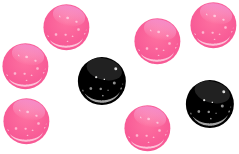
\includegraphics[height=2.6cm,keepaspectratio]{assets/iconqa_item_38.png}

{\scriptsize IconQA item 38, train split}
\column{0.60\textwidth}
\raggedright\scriptsize
If you select a marble without looking, how likely is it that you will pick a black one?\\[2pt]
A. unlikely \quad B. probable \quad C. certain \quad D. impossible\\[2pt]
Respond with only the option label.\\
Answer:

\vspace{0.22cm}
\renewcommand{\arraystretch}{1.05}
\begin{tabular}{@{}lrrr@{}}
\toprule
Accuracy, image + A/B/C/D (\%) & Qwen & InternVL & LLaVA \\
\midrule
Confirmation pairs & 99.2 & 95.1 & 95.1 \\
\bottomrule
\end{tabular}

\vspace{0.14cm}
\fontsize{7.6}{9.2}\selectfont
The models solve this narrow task reliably when the image is present.\par
\vspace{0.06cm}
\textbf{Scope.} From IconQA's text-option multiple-choice questions we used one task, marble probability, and created counterfactual pairs for it as we did for CLEVR: 8 calibration, 64 discovery and 64 confirmation pairs, of which each model uses 32 correctly answered pairs per phase.
\end{columns}
\end{frame}

%======================================================================
\sectionslide{Methods}

\begin{frame}{Activation patching}
\begin{columns}[T,onlytextwidth]
\column{0.40\textwidth}
\centering
\begin{minipage}[t]{0.48\linewidth}\centering
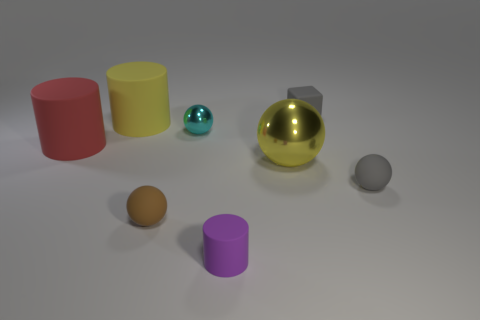
\includegraphics[width=\linewidth]{assets/clevr_pair_x.png}\\[1pt]
{\scriptsize donor: answer \textbf{A}}
\end{minipage}\hfill
\begin{minipage}[t]{0.48\linewidth}\centering
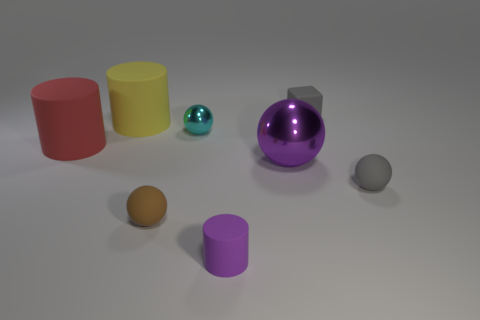
\includegraphics[width=\linewidth]{assets/clevr_pair_y.png}\\[1pt]
{\scriptsize recipient: answer \textbf{D}}
\end{minipage}

\vspace{0.12cm}
\begin{minipage}{\linewidth}\raggedright\tiny
What color is the large sphere that is in front of the yellow cylinder?\\
A. yellow \quad B. gray \quad C. red \quad D. purple\\
Respond with only the option label. Answer:
\end{minipage}

\vspace{0.16cm}
\begin{minipage}{\linewidth}\raggedright\scriptsize
\textbf{Donor:} the run we copy an internal activation from.\\[2pt]
\textbf{Recipient:} the run we insert it into.
\end{minipage}

\column{0.57\textwidth}
\centering
{\footnotesize\textbf{A prompt has four token groups}}\par
\vspace{0.10cm}
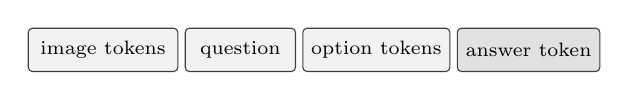
\begin{tikzpicture}[font=\scriptsize,
  tok/.style={draw=Ink,rounded corners=1.5pt,minimum height=0.55cm,inner sep=3pt,align=center,fill=Mist}]
\node[tok,minimum width=1.9cm] (i) {image tokens};
\node[tok,minimum width=1.4cm,right=0.08cm of i] (q) {question};
\node[tok,minimum width=1.7cm,right=0.08cm of q] (o) {option tokens};
\node[tok,minimum width=1.4cm,right=0.08cm of o,fill=Gold!45] (a) {answer token};
\end{tikzpicture}\par
\vspace{0.10cm}
{\scriptsize Different methods patch different sets of these tokens, at a chosen subset of layers and attention heads.\par}

\vspace{0.18cm}
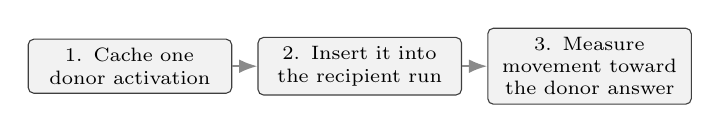
\begin{tikzpicture}[node distance=0.32cm,>=Latex,
  st/.style={draw=Ink,fill=Mist,rounded corners=2pt,text width=2.35cm,minimum height=0.62cm,align=center,font=\scriptsize}]
\node[st] (a) {1. Cache one donor activation};
\node[st,right=of a] (b) {2. Insert it into the recipient run};
\node[st,right=of b] (c) {3. Measure movement toward the donor answer};
\draw[->,Slate,thick] (a) -- (b);
\draw[->,Slate,thick] (b) -- (c);
\end{tikzpicture}

\vspace{0.22cm}
{\small$\displaystyle
\mathrm{Recovery}=\frac{s_{\mathrm{patched}}-s_{\mathrm{recipient}}}{s_{\mathrm{donor}}-s_{\mathrm{recipient}}}$}

\vspace{0.06cm}
{\scriptsize $s$ is the logit difference between the two answers. $0$: no movement; $1$: full donor transfer.\par}
\end{columns}
\source{Final report Figure 6, CLEVR scene 047521}
\end{frame}

%======================================================================
\sectionslide{Core-7}

\begin{frame}{Logit Lens vs. Tuned Lens}
\begin{columns}[T,onlytextwidth]
\column{0.47\textwidth}
\centering{\footnotesize\bfseries LOGIT LENS\par}
\vspace{0.12cm}
\raggedright\fontsize{7.8}{9.6}\selectfont
\textbf{What it does.} Takes the hidden state at the answer token after a layer and decodes it with the model's final unembedding matrix, as if that layer were the last one. No training.

\vspace{0.12cm}
\textbf{What it is useful for.} Following, layer by layer, when the answer label, the content word or the requested alphabet becomes readable (M4, M5, M7).

\vspace{0.12cm}
\textbf{Its limit.} Middle layers are not yet in the final embedding space, so information can be present but unreadable, and milestones can look later than they are.
\column{0.02\textwidth}
\centering{\color{Gold}\rule{0.4pt}{5.2cm}}
\column{0.47\textwidth}
\centering{\footnotesize\bfseries TUNED LENS\par}
\vspace{0.12cm}
\raggedright\fontsize{7.8}{9.6}\selectfont
\textbf{How it differs.} Before decoding, it passes each layer's hidden state through a small learned translator that maps it into the final embedding space.

\vspace{0.12cm}
\textbf{What it is useful for.} A more faithful layer-by-layer readout, so we can check whether a Logit Lens milestone is real or just an artefact of reading a middle layer as if it were the last.

\vspace{0.12cm}
\textbf{What we did.} For each model we trained one translator per layer, teaching it to predict what the model finally outputs. We trained on separate CLEVR scenes that are never used for evaluation. After training, middle layers predict the final output far more closely than with the Logit Lens.
\end{columns}
\end{frame}

\begin{frame}{Methods Overview}
\begin{columns}[T,onlytextwidth]
\column{0.52\textwidth}
\raggedright
{\footnotesize\bfseries CAUSAL INTERVENTIONS\par}
{\fontsize{6.8}{8.2}\selectfont\color{Slate}copy activations from a donor run into a recipient run\par}
\vspace{0.14cm}
\methoditem{M1}{When can a donor answer steer the output?}{Patch the final-token state from a donor into a recipient, one layer at a time.}
\methoditem{M2}{Does attention or the MLP matter more?}{Patch attention and MLP activations separately, to see which matters more.}
\methoditem{M3}{Do a few attention heads dominate?}{Rank individual attention heads on discovery and freeze each top-$k$ set.}
\methoditem{M6}{Which token groups carry the effect?}{Patch image, question, option and label token groups separately. Identifies which tokens carry the transferable answer content.}
\column{0.02\textwidth}
\centering
{\color{Gold}\rule{0.4pt}{5.7cm}}
\column{0.42\textwidth}
\raggedright
{\footnotesize\bfseries OBSERVATIONAL READOUTS\par}
{\fontsize{6.8}{8.2}\selectfont\color{Slate}project internal states onto the vocabulary; nothing is patched\par}
\vspace{0.14cm}
\methoditem{M4}{When is the answer label readable?}{Project each residual state to the output vocabulary using the Logit Lens and the Tuned Lens.}
\methoditem{M5}{Is content readable before the symbol?}{Compare the semantic answer word with its printed label through depth. Shows which becomes readable first at the final token.}
\methoditem{M7}{Do unfamiliar labels change the route?}{Repeat behaviour and readouts across A/B/C/D, 1/2/3/4 and Q/Z/R/X. Tracks when the requested alphabet overtakes default A/B/C/D directions.}
\end{columns}
\end{frame}


\begin{frame}{M4: When is the answer label readable?}
\begin{columns}[T,onlytextwidth]
\column{0.42\textwidth}
\raggedright\fontsize{7.4}{9}\selectfont
\textbf{Question}\par \emph{At what depth does the model know which label to print?}

\vspace{0.12cm}
\textbf{What we did}\par At the final (``Answer:'') token we project the residual state after every layer onto the vocabulary with both lenses, on the behaviour split and for all three alphabets. We track the probability of the correct label among the four shown labels, and how much of the vocabulary goes to those labels. ``Readable'' is the first stage where the correct-minus-wrong margin and its lower bound are above zero.

\vspace{0.12cm}
\textbf{Results}\par First readable stage (A/B/C/D), Logit\,/\,Tuned: Qwen 22\,/\,20 of 28; InternVL 25\,/\,25 of 36; LLaVA 25\,/\,20 of 28; PaliGemma 35\,/\,35 of 42. The big jump in correct-label probability sits at the same stage under both lenses.
\column{0.55\textwidth}
\centering
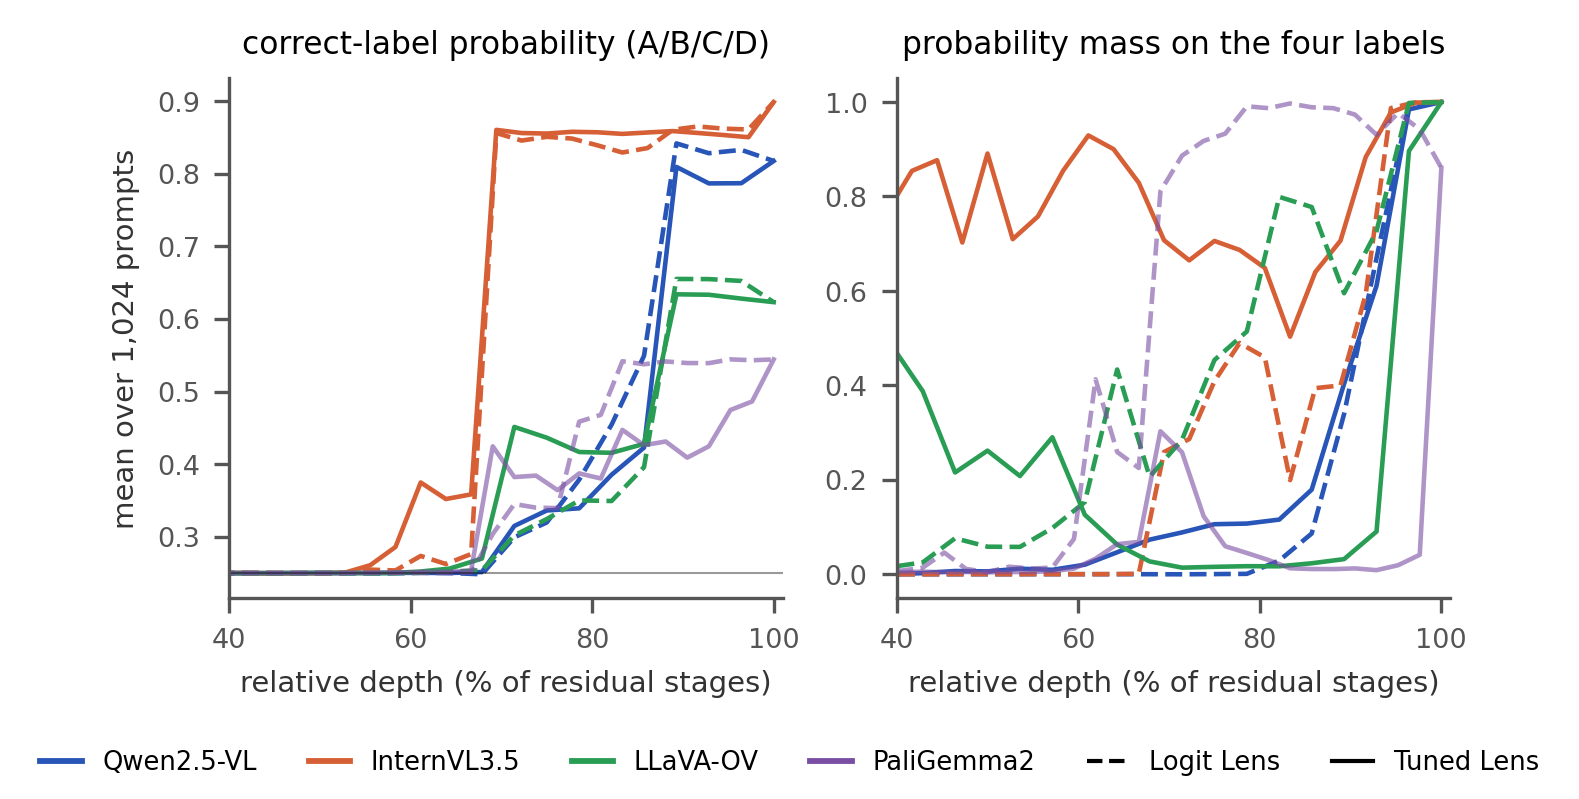
\includegraphics[width=\linewidth]{assets/core7_m4.png}\par
\vspace{0.10cm}
\raggedright
\lesson{\textbf{What we learned.} In all four models the label decision is \emph{late} (about 70--90\% depth), and the Tuned Lens does not move it, so there is no hidden early answer. With rare letters the label becomes readable at the same depth or slightly later. Tuned Lens results are more consistent across models.}
\end{columns}
\end{frame}

\begin{frame}{M5: Is content readable before the symbol?}
\begin{columns}[T,onlytextwidth]
\column{0.42\textwidth}
\raggedright\fontsize{7.4}{9}\selectfont
\textbf{Question}\par \emph{Does the answer token carry the answer's meaning first and then convert it to a symbol, or the reverse?}

\vspace{0.12cm}
\textbf{What we did}\par At every layer, using both lenses, we compare two margins at the answer token: the \emph{label margin} (correct label vs.\ best wrong label) and the \emph{content-word margin} (the correct answer word, e.g.\ ``yellow'', vs.\ the best wrong answer word).

\vspace{0.12cm}
\textbf{Results}\par Content word first readable, Logit\,/\,Tuned: Qwen 27\,/\,28; InternVL 27\,/\,34; LLaVA 27\,/\,28; PaliGemma never (negative at every stage, $-0.08$ at its output). The label is readable earlier: 22, 25, 25 and 35 under the Logit Lens.
\column{0.55\textwidth}
\centering
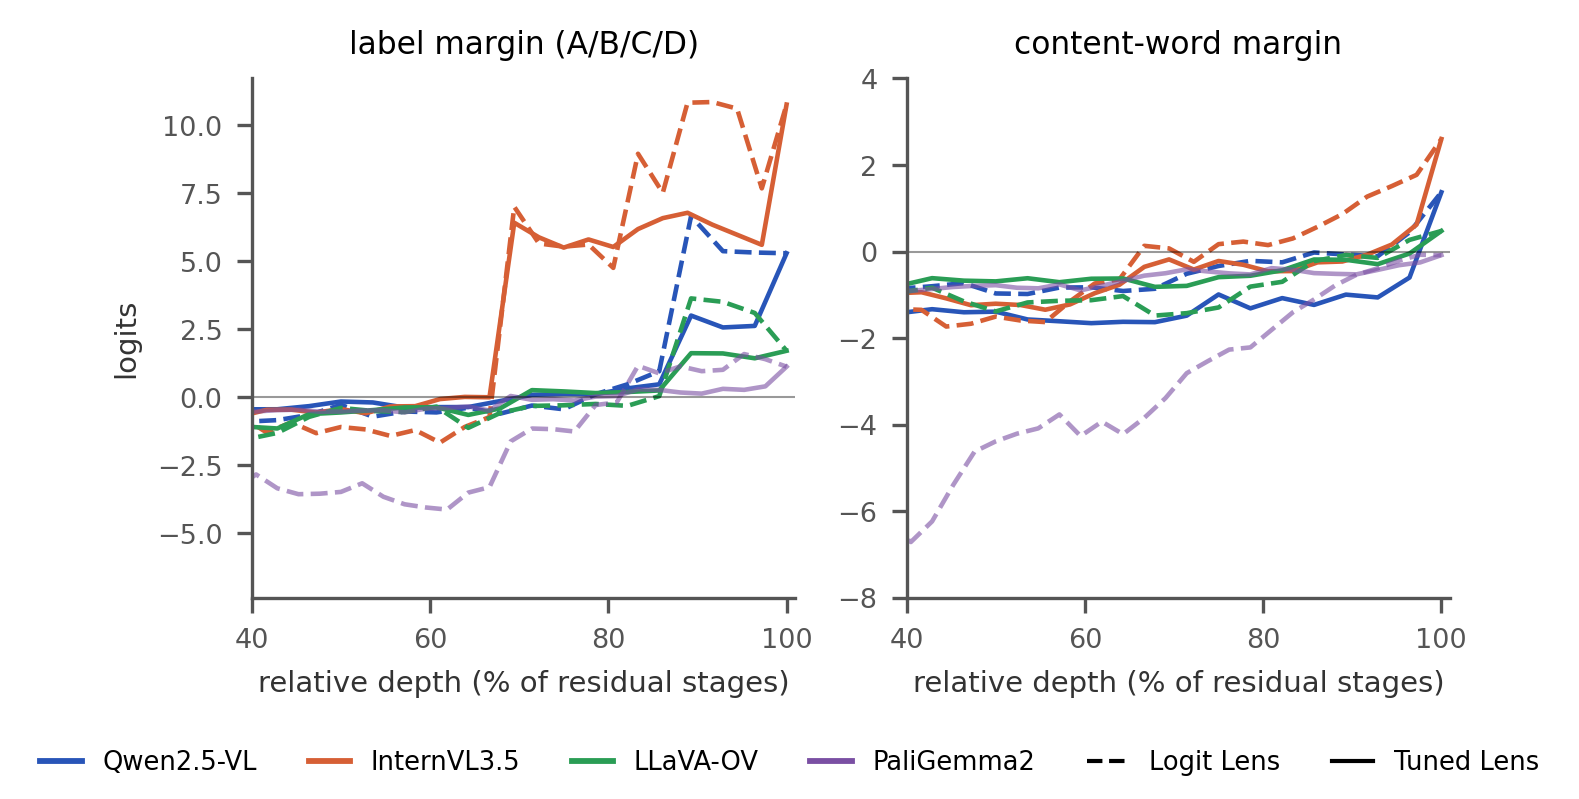
\includegraphics[width=\linewidth]{assets/core7_m5.png}\par
\vspace{0.10cm}
\raggedright
\lesson{\textbf{What we learned.} At the answer token the \emph{label} becomes readable before, or together with, the content word in every model, under both lenses: this position carries the symbol to print, not the answer word.}
\end{columns}
\end{frame}

\begin{frame}{M7: Do unfamiliar labels change the route?}
\begin{columns}[T,onlytextwidth]
\column{0.42\textwidth}
\raggedright\fontsize{7.4}{9}\selectfont
\textbf{Question}\par \emph{Does the model first think in A/B/C/D and switch to the requested alphabet only at the end?}

\vspace{0.12cm}
\textbf{What we did}\par At every layer we repeat behaviour and both lens readouts with 1/2/3/4 and the rare letters Q/Z/R/X, and measure the share of probability on the \emph{requested} labels versus the default A/B/C/D.

\vspace{0.12cm}
\textbf{Results}\par Accuracy barely changes with the alphabet (A/B/C/D\,/\,numbers\,/\,rare: Qwen 84/80/82\%, InternVL 91/78/86\%, LLaVA 65/64/63\%, PaliGemma 54/53/53\%). Logit Lens: the rare alphabet holds almost no share until the decision, then jumps within a single stage: Qwen 0.13\,$\rightarrow$\,0.83, InternVL 0.07\,$\rightarrow$\,0.98, LLaVA 0.01\,$\rightarrow$\,0.72, PaliGemma 0.08\,$\rightarrow$\,0.88. Tuned Lens: in the same middle layers the share is already high (InternVL 0.89--0.96, LLaVA 0.44--0.73, Qwen 0.29--0.51; PaliGemma only 0.1--0.3), so the late jump is much smaller.
\column{0.55\textwidth}
\centering
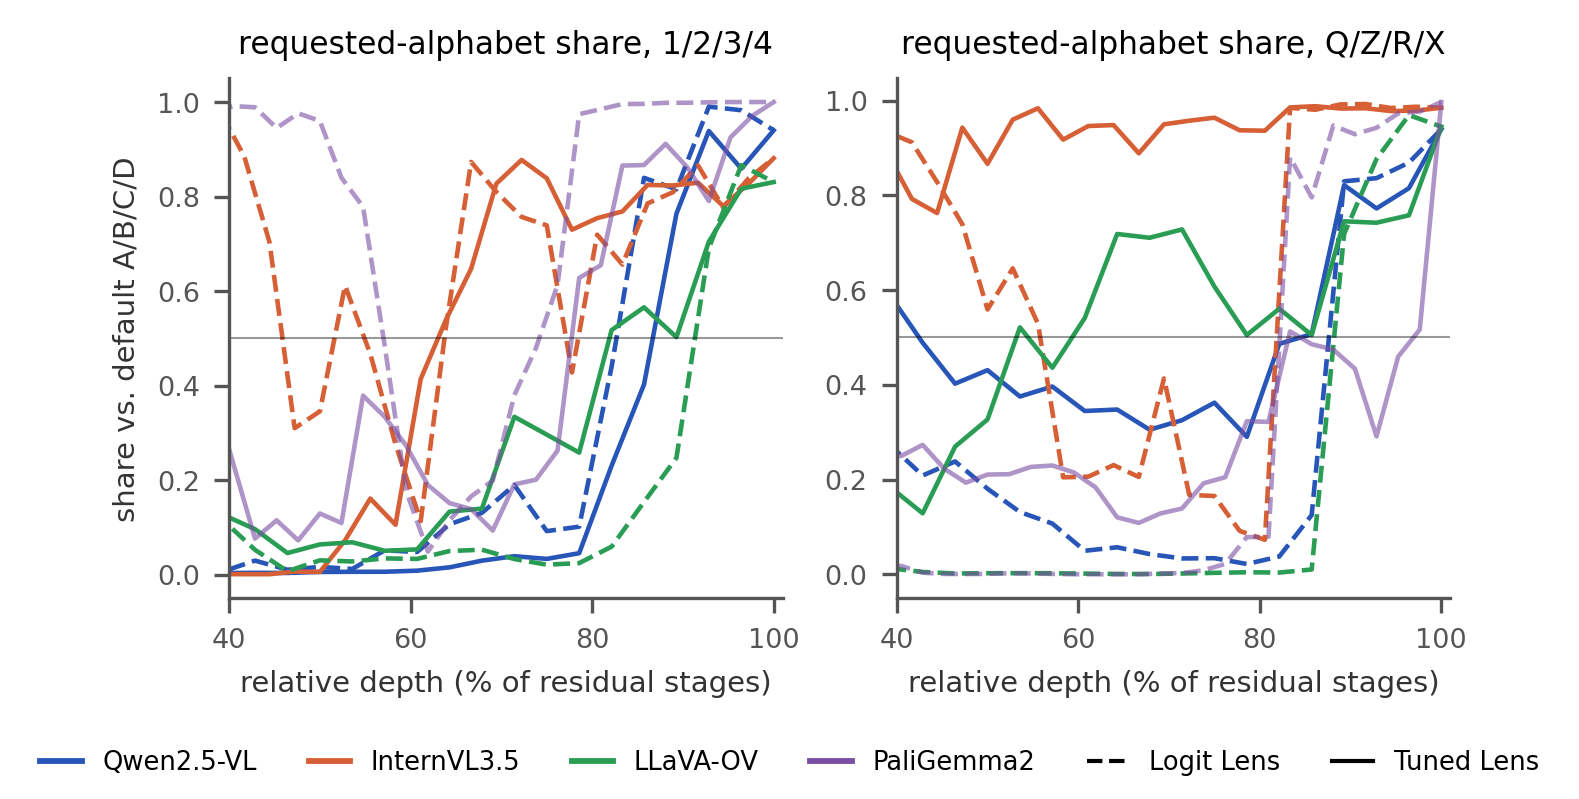
\includegraphics[width=\linewidth]{assets/core7_m7.png}\par
\vspace{0.10cm}
\raggedright
\lesson{\textbf{What we learned.} The Logit Lens shows the requested alphabet appearing suddenly at the very end, while the Tuned Lens shows it building up gradually and gives it a much higher share in the middle layers. So the model has already chosen which alphabet to answer in well before the end. The model's own unembedding matrix just cannot recover that choice from the middle layers, while the trained Tuned Lens can.}
\end{columns}
\end{frame}

\begin{frame}{M1: When can a donor answer steer the output?}
\begin{columns}[T,onlytextwidth]
\column{0.42\textwidth}
\raggedright\fontsize{7.4}{9}\selectfont
\textbf{Question}\par \emph{From which layer does the final token carry a portable answer?}

\vspace{0.12cm}
\textbf{What we did}\par At every layer we copy the donor's full residual state at the final token into the recipient and measure recovery toward the donor's answer (0 = none, 1 = full), for position, content and random-pair (control) contrasts. The transfer layer, the first with mean recovery $\ge$ 0.5, is frozen on discovery and re-tested on confirmation.

\vspace{0.12cm}
\textbf{Results}\par Position\,/\,content transfer layer: Qwen 24\,/\,25; InternVL 29\,/\,31; LLaVA 24\,/\,23; PaliGemma 37\,/\,37. The exact order replicates in Qwen and InternVL, not in LLaVA or PaliGemma. Random pairs also cross 0.5 (layers 24, 25, 24, 39).
\column{0.55\textwidth}
\centering
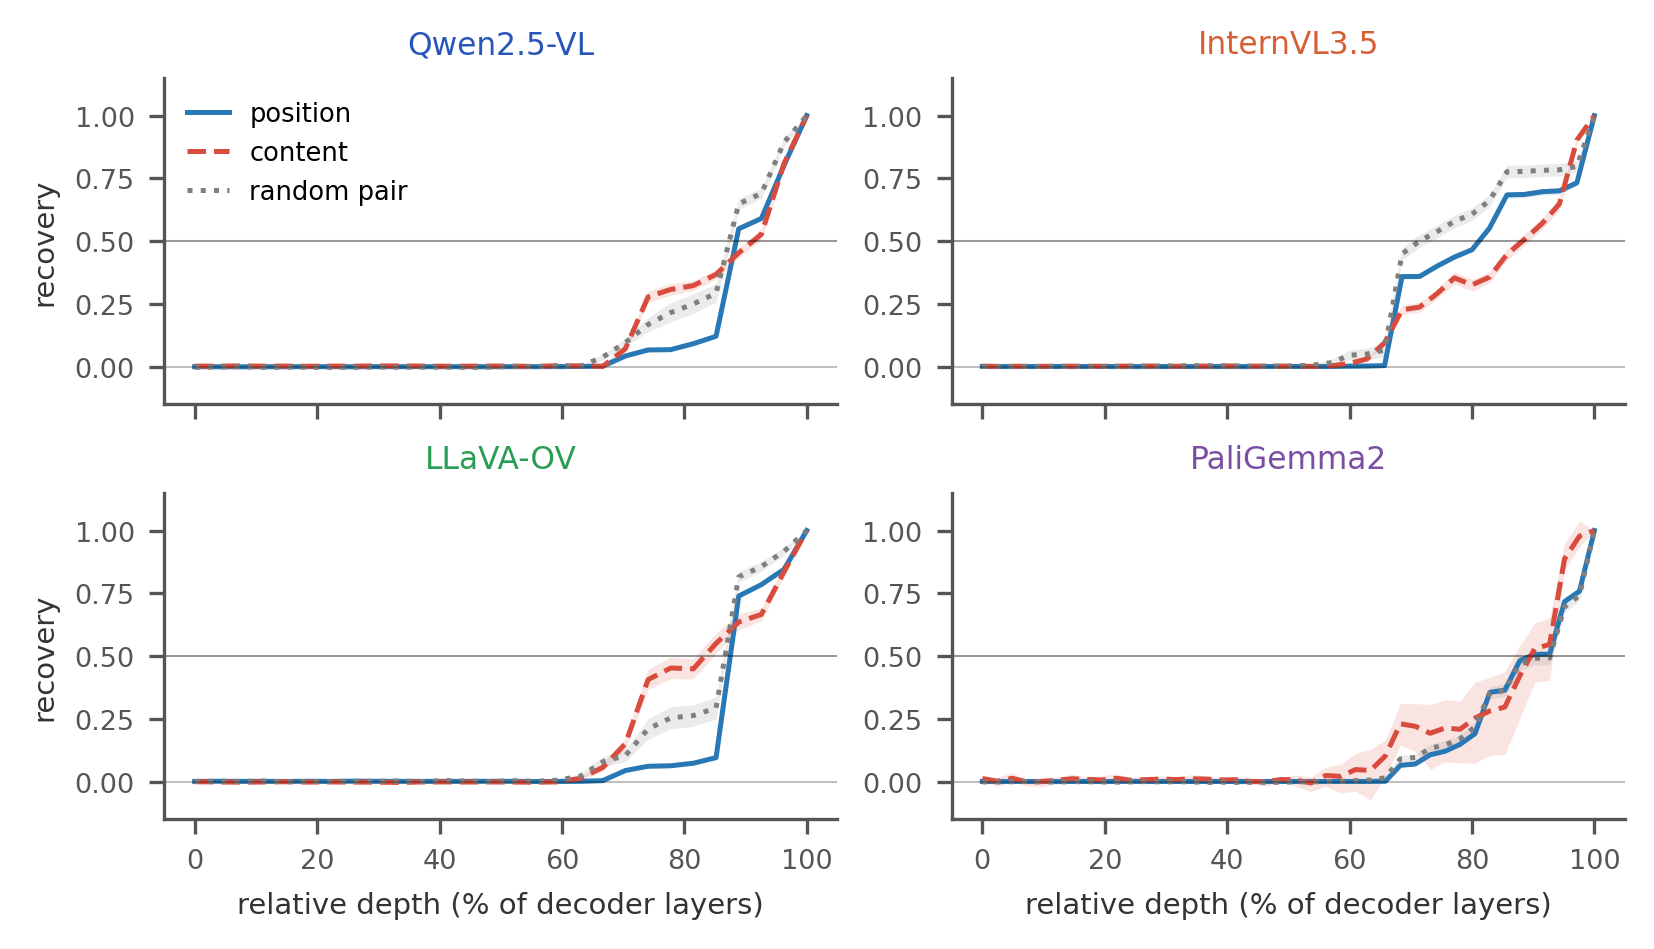
\includegraphics[width=\linewidth]{assets/core7_m1.png}\par
\vspace{0.10cm}
\raggedright
\lesson{\textbf{What we learned.} In all four models the final token holds no answer until about 65--85\% depth, then a portable answer state appears and fully transfers by the last layer. Random donors transfer as strongly, so it is a generic answer state, not specific to counterfactual pairs. This shows that towards the late layers, models encode a transferable answer symbol in the final token.}
\end{columns}
\end{frame}

\begin{frame}{M2: Does attention or the MLP matter more?}
\begin{columns}[T,onlytextwidth]
\column{0.42\textwidth}
\raggedright\fontsize{7.4}{9}\selectfont
\textbf{Question}\par \emph{Which component writes the answer into the final token?}

\vspace{0.12cm}
\textbf{What we did}\par At every layer, at the final token, we replace the attention output or the MLP output with the donor's (position contrasts) and measure recovery, as in the plot. As a second check, we replace each component's output with its output from an unrelated example, and measure how much the model's lead for its correct answer (correct-label logit minus the best wrong label) falls.

\vspace{0.12cm}
\textbf{Results}\par Peak recovery, attention vs.\ MLP: Qwen 0.44 vs.\ 0.11, InternVL 0.35 vs.\ 0.05, LLaVA 0.64 vs.\ 0.10 (all at layer 24); PaliGemma 0.22 (L41) vs.\ 0.15 (L39). Replacing layer-24 attention this way cuts the correct answer's lead by 4.4, 5.6 and 5.0 logits; replacing the layer-24 MLP cuts it by only 0.5, 0.1 and 0.6 (PaliGemma: 2.3 for L41 attention vs.\ 1.4 for L39 MLP).
\column{0.55\textwidth}
\centering
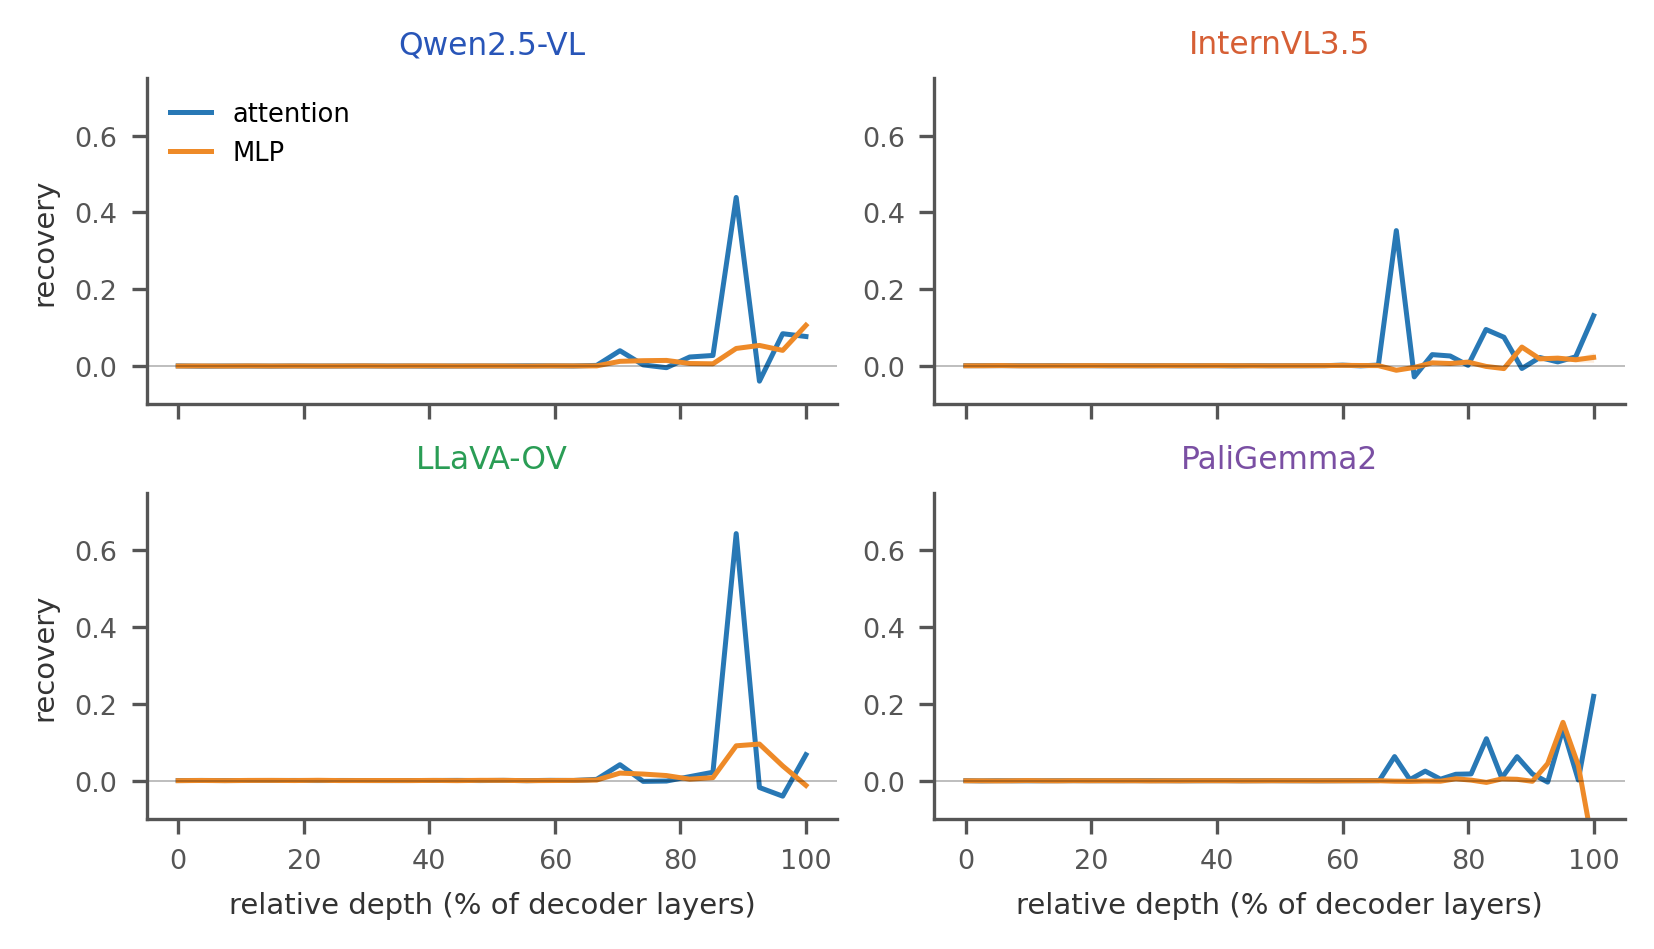
\includegraphics[width=\linewidth]{assets/core7_m2.png}\par
\vspace{0.10cm}
\raggedright
\lesson{\textbf{What we learned.} Late answer transfer is \emph{attention-dominated} in all four models: a late attention layer moves the answer into the final position. In the three Qwen-lineage models this is one sharp layer (24); PaliGemma spreads it over its last layers and gives the MLP a larger share.}
\end{columns}
\par\vfill{\fontsize{6}{7}\selectfont\color{Slate}Attention or MLP output patching replaces only the output of that module at one layer. Normal activation patching (M1) replaces the residual stream, i.e.\ the state after both the attention output and the MLP output have been added.\par}
\end{frame}

\begin{frame}{M3: Do a few attention heads dominate?}
\begin{columns}[T,onlytextwidth]
\column{0.42\textwidth}
\raggedright\fontsize{7.4}{9}\selectfont
\textbf{Question}\par \emph{Is the late attention effect carried by a handful of heads?}

\vspace{0.12cm}
\textbf{What we did}\par In the four strongest attention layers (Qwen 19, 24, 26, 27; InternVL 24, 29, 30, 35; LLaVA 19, 23, 24, 27; PaliGemma 28, 34, 39, 41) we run the model patching one head at a time on discovery, rank the heads, and freeze the top-$k$ sets ($k$ = 1 to 16). On confirmation each set is compared with 20 random head sets of the same size and layers. The random baseline is their 95th percentile: the score that only the best 5\% of random sets reach. ``Sparse'': four or fewer heads already recover at least 50\% of the all-head effect.


\vspace{0.12cm}
\textbf{Results}\par Top-4 heads vs.\ the random 95th percentile: 0.42 vs.\ 0.07 (Qwen), 0.44 vs.\ 0.09 (InternVL), 0.58 vs.\ 0.03 (LLaVA), 0.62 vs.\ 0.01 (PaliGemma), i.e.\ 53, 52, 71 and 93\% of the all-head effect. Sparse in all but InternVL, which crosses the 50\% line between phases.
\column{0.55\textwidth}
\centering
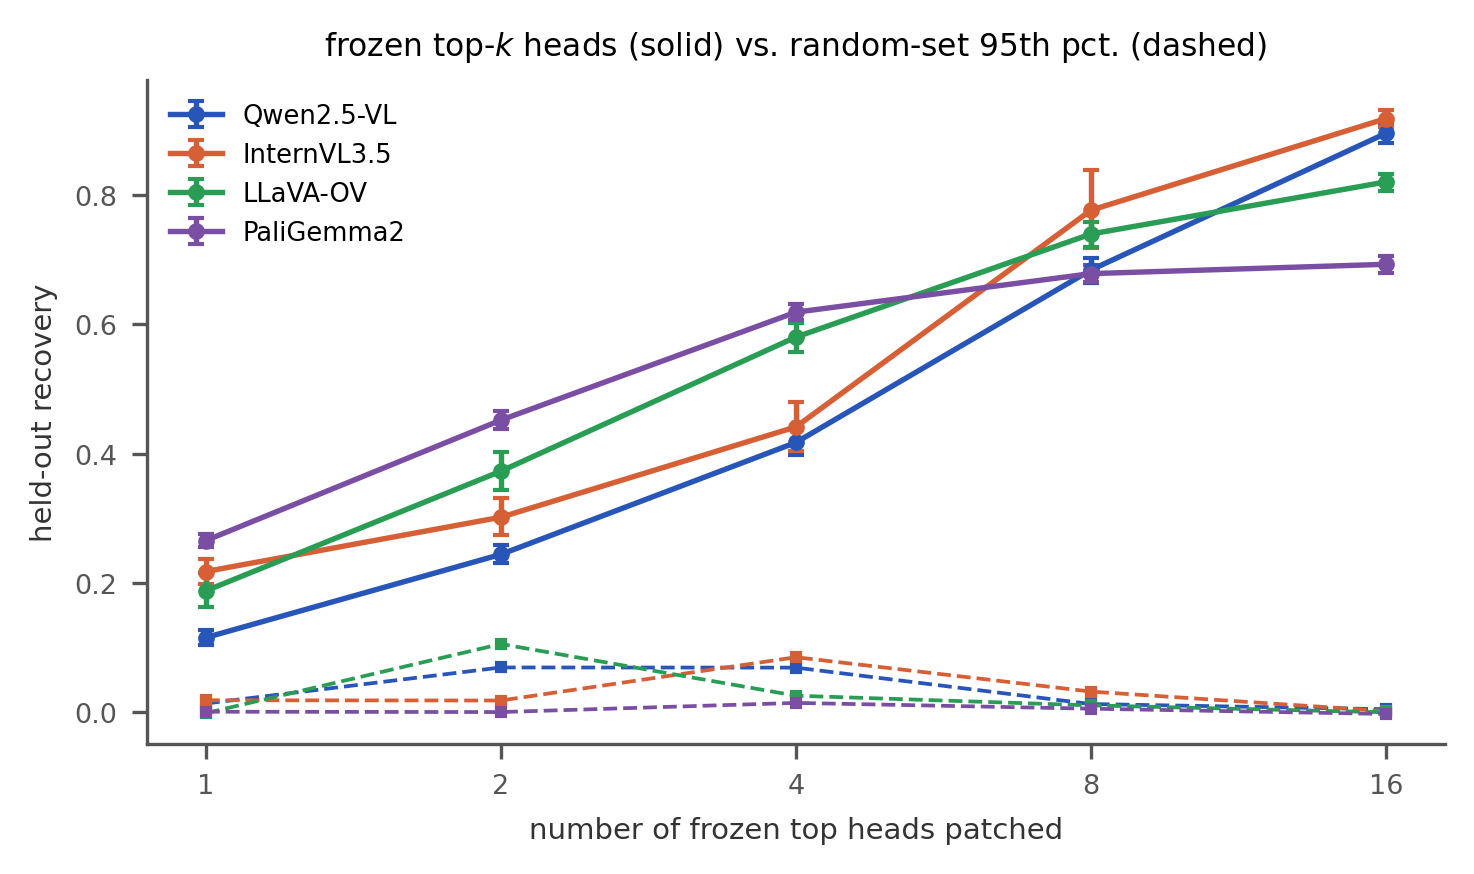
\includegraphics[width=\linewidth]{assets/core7_m3.png}\par
\vspace{0.10cm}
\raggedright
\lesson{\textbf{What we learned.} In every model a few frozen heads carry a large share of the answer transfer: even against the best 5\% of random head sets, the selected top-$k$ sets win by a large margin. These are consistent late ``answer-mover'' heads. How sparse they are varies by model, and they are useful heads, not a complete or unique circuit.}
\end{columns}
\end{frame}

\begin{frame}{M6: Which token groups carry the effect?}
\begin{columns}[T,onlytextwidth]
\column{0.42\textwidth}
\raggedright\fontsize{7.4}{9}\selectfont
\textbf{Question}\par \emph{Where in the prompt does the answer content live at each depth?}

\vspace{0.12cm}
\textbf{What we did}\par At every second layer, on content contrasts, we replace the residual states of one whole token group (image, question, option contents or option labels) with the donor's, and measure recovery at the output.

\vspace{0.12cm}
\textbf{Results}\par Image tokens restore almost the full effect up to about 40--50\% depth in all four models. Option contents then peak mid-depth: Qwen 0.42 (L18), InternVL 0.24 (L22), LLaVA 0.53 (L18), PaliGemma 0.77 (L26). Question tokens carry less; label tokens carry almost nothing.
\column{0.55\textwidth}
\centering
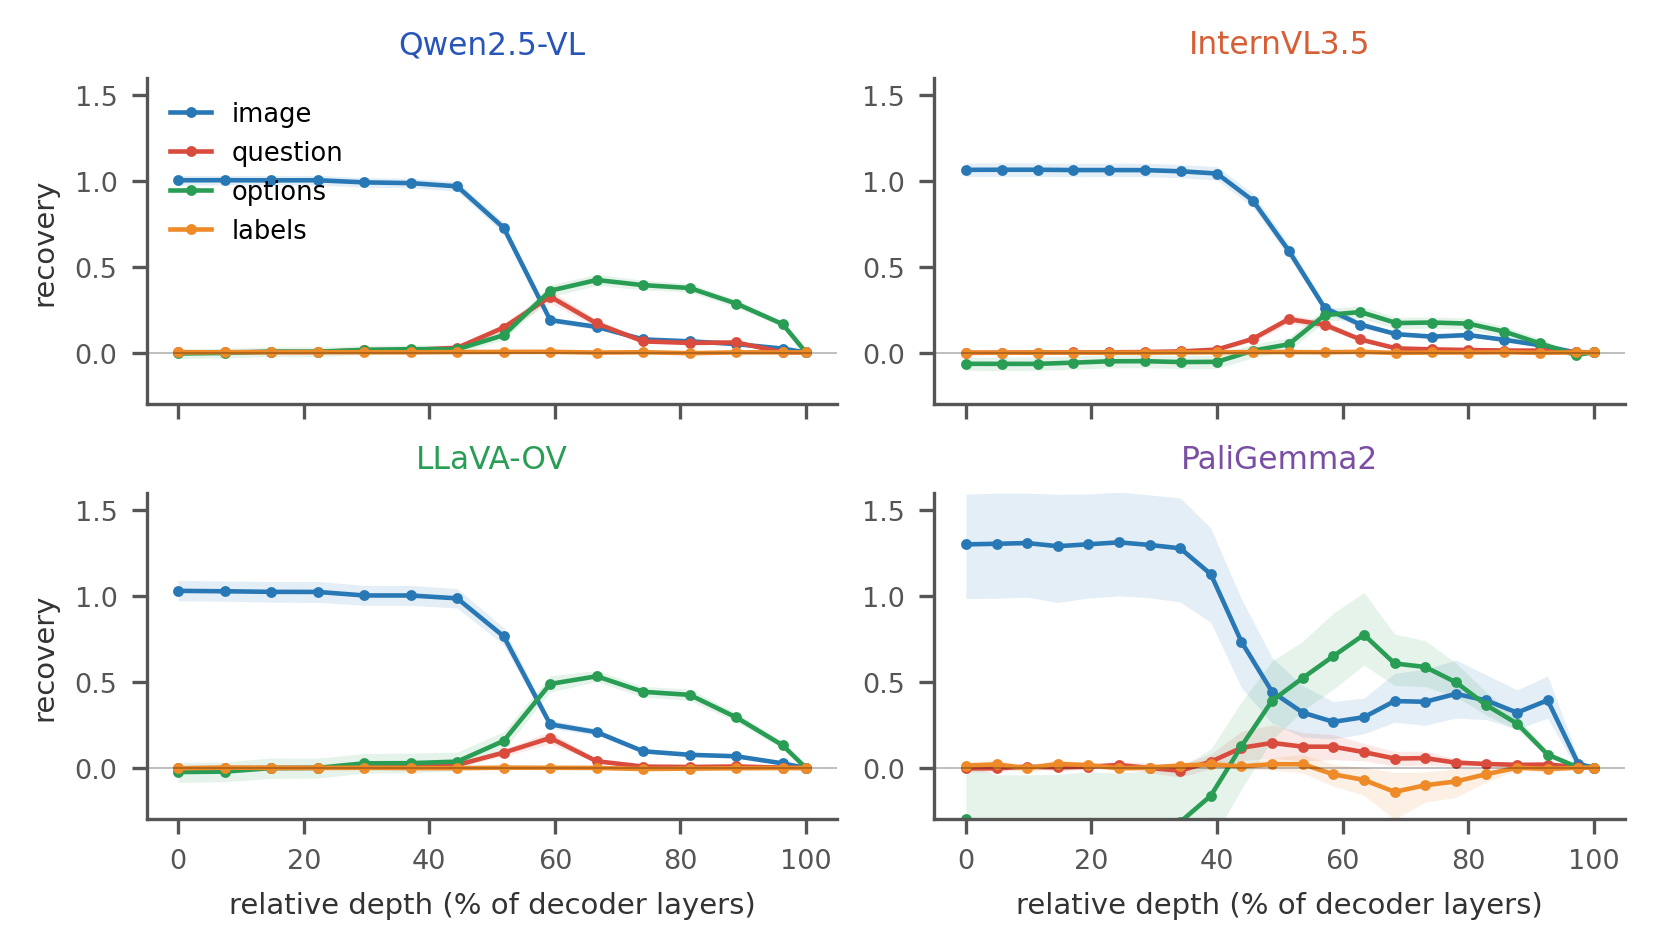
\includegraphics[width=\linewidth]{assets/core7_m6.png}\par
\vspace{0.10cm}
\raggedright
\lesson{\textbf{What we learned.} The answer content moves from the \emph{image tokens} to the \emph{option and question tokens} in the middle layers, and then to the final token (M1--M3). This staged route holds in all four models. PaliGemma's curves are noisier, so the route is broad, not edge-precise. The label tokens never carry the content.}
\end{columns}
\end{frame}

\begin{frame}{IconQA: does Core-7 transfer?}
\centering
{\fontsize{7.4}{9}\selectfont Core-7 re-run on 32 correctly answered IconQA pairs per phase (lens readouts: Logit Lens only; PaliGemma: changed prompt). Values: Qwen\,/\,InternVL\,/\,LLaVA\,/\,PaliGemma.\par}
\vspace{0.06cm}
\fontsize{6.7}{8}\selectfont
\renewcommand{\arraystretch}{1.0}
\begin{tabularx}{\textwidth}{@{}>{\bfseries\raggedright\arraybackslash}p{2.45cm}>{\raggedright\arraybackslash}p{3.1cm}>{\raggedright\arraybackslash}X>{\raggedright\arraybackslash}p{2.25cm}@{}}
\toprule
Method & On CLEVR & On IconQA & Transfers? \\
\midrule
M4\newline Label readable & Late: stage 22\,/\,25\,/\,25\,/\,35 & Late again: stage 21\,/\,25\,/\,20\,/\,29 & \textbf{Yes} \\
M5\newline Content vs.\ label & Label first; content word at 27\,/\,27\,/\,27\,/\,never & Label first; content word at 28\,/\,34\,/\,never\,/\,34 & \textbf{Yes} \\
M7\newline Alphabet & Logit Lens: sudden jump at the end & The same sudden late jump (e.g.\ Qwen rare letters 0.13\,$\rightarrow$\,0.89 at stage 25) & \textbf{Yes} \\
M1\newline Final-token transfer & Late, portable; position first in Qwen, InternVL & Late again; content before position in InternVL, LLaVA and PaliGemma & \textbf{Partly}: late transfer yes, order no \\
M2\newline Attention vs.\ MLP & Attention dominates (layer 24) & Attention 0.46\,/\,0.25\,/\,0.67\,/\,0.24 vs.\ MLP 0.15\,/\,0.06\,/\,0.08\,/\,0.13 & \textbf{Yes} \\
M3\newline Heads & Top-4 carry 53\,/\,52\,/\,71\,/\,93\% & IconQA top-4: 53\,/\,52\,/\,74\,/\,92\%; CLEVR heads reused: 53\,/\,49.6\,/\,74\,/\,92\% & \textbf{Yes} \\
M6\newline Token groups & Image early; options, question mid-depth & Image and option tokens at the input, question mid-depth; PaliGemma's image effect peaks late & \textbf{Mostly}; PaliGemma differs \\
\bottomrule
\end{tabularx}

\vspace{0.08cm}
\raggedright
\lesson{\textbf{What we learned.} Almost everything transfers: late label readability, label before content, the late alphabet jump, attention-dominated answer writing and small answer-mover heads, even those chosen on CLEVR. The order of content and position does not.}
\end{frame}

%======================================================================
\sectionslide{Extended Experiments}

\begin{frame}{Extended Experiments Overview}
\begin{columns}[T,onlytextwidth]
\column{0.48\textwidth}
\raggedright
\methoditem{S1}{Does image information flow through the heads?}{Keep the text fixed and change only the image: restore early image states, copy the frozen top-4 heads, or clamp them.}
\methoditem{S2}{Can a wrong printed symbol be repaired?}{A screen of saved records finds errors with the right content but the wrong symbol; S2 patches option states from a same-image donor to repair them.}
\column{0.48\textwidth}
\raggedright
\methoditem{S3}{Do the heads route to specific image regions?}{Block the heads' attention to the question-object or option-object region and compare with an equal-size control region.}
\methoditem{S4}{With image answer options, content or symbol?}{Show the question and options as image panels; test whether the heads move the donor's visual content or copy its printed symbol.}
\end{columns}

\vspace{0.30cm}
\centering
{\color{Rule}\rule{0.72\textwidth}{0.4pt}\par}
\vspace{0.14cm}
{\fontsize{7.6}{9.2}\selectfont Core-7 finds useful sites; these studies test how they connect. All four run on CLEVR scenes with each model's own frozen Core-7 top-4 heads, 20 random 4-head sets as control, one layer or site frozen on discovery and tested once on held-out scenes. Models: Qwen, InternVL and LLaVA (PaliGemma not run).\par}
\end{frame}

\begin{frame}{Extended experiments: data and inputs}
\scriptsize
\renewcommand{\arraystretch}{1.25}
\begin{tabularx}{\textwidth}{@{}>{\bfseries}p{0.9cm}>{\raggedright\arraybackslash}X>{\raggedright\arraybackslash}X>{\raggedright\arraybackslash}p{3.4cm}@{}}
\toprule
Study & Data & Input change & What we score \\
\midrule
S1 & The same CLEVR counterfactual pairs, keeping only pairs where every direction also has its matched controls & Donor and recipient prompts are identical in text; only the image differs & Effect on the donor's answer (logits) \\
S2 & The model's own errors from the behaviour split (found by a screen of saved records), plus matched already-correct scenes as controls & The recipient is a wrong answer; the donor is the same image with the options rearranged & The recipient's truth margin and \% of errors fixed \\
S3 & CLEVR scenes chosen from their scene graphs: two uniquely described objects, so the question can name either & Object bounding boxes are mapped onto the image tokens to form regions & Answer change when a region is blocked, minus a control region \\
S4 & Objects cropped from CLEVR scenes into one collage: a query panel above four option panels A--D & The options are images, not words; the query panel equals one option & Move toward the donor's content minus copying its symbol \\
\bottomrule
\end{tabularx}
\end{frame}

\begin{frame}{S1: Does image information flow through the heads?}
\begin{columns}[T,onlytextwidth]
\column{0.42\textwidth}
\raggedright\fontsize{7.4}{9}\selectfont
\textbf{Question}\par \emph{With the prompt fixed and only the image changed, does restoring early image states bring back the donor's answer, and do the frozen heads carry that effect?}


\vspace{0.12cm}
\textbf{What we did}\par Donor and recipient share the exact same text and differ only in the image. We (1) replace all image-token states at layer 0 with the donor's, (2) copy only the frozen top-4 heads' outputs at the final token, and (3) restore the image while clamping those four heads to their recipient values. Heads are compared with 20 random 4-head sets from the same layers.

\vspace{0.12cm}
\textbf{Results}\par Image restoration recovers the full donor effect: +24.0 logits in Qwen and +40.2 in InternVL (recovery 1.00). Copying the four heads moves the answer by +9.7 (Qwen) and +17.7 logits (InternVL), against about 0 for random heads; clamping them removes almost the same amount. LLaVA: we were not able to run it on this model in the stipulated time.
\column{0.55\textwidth}
\centering
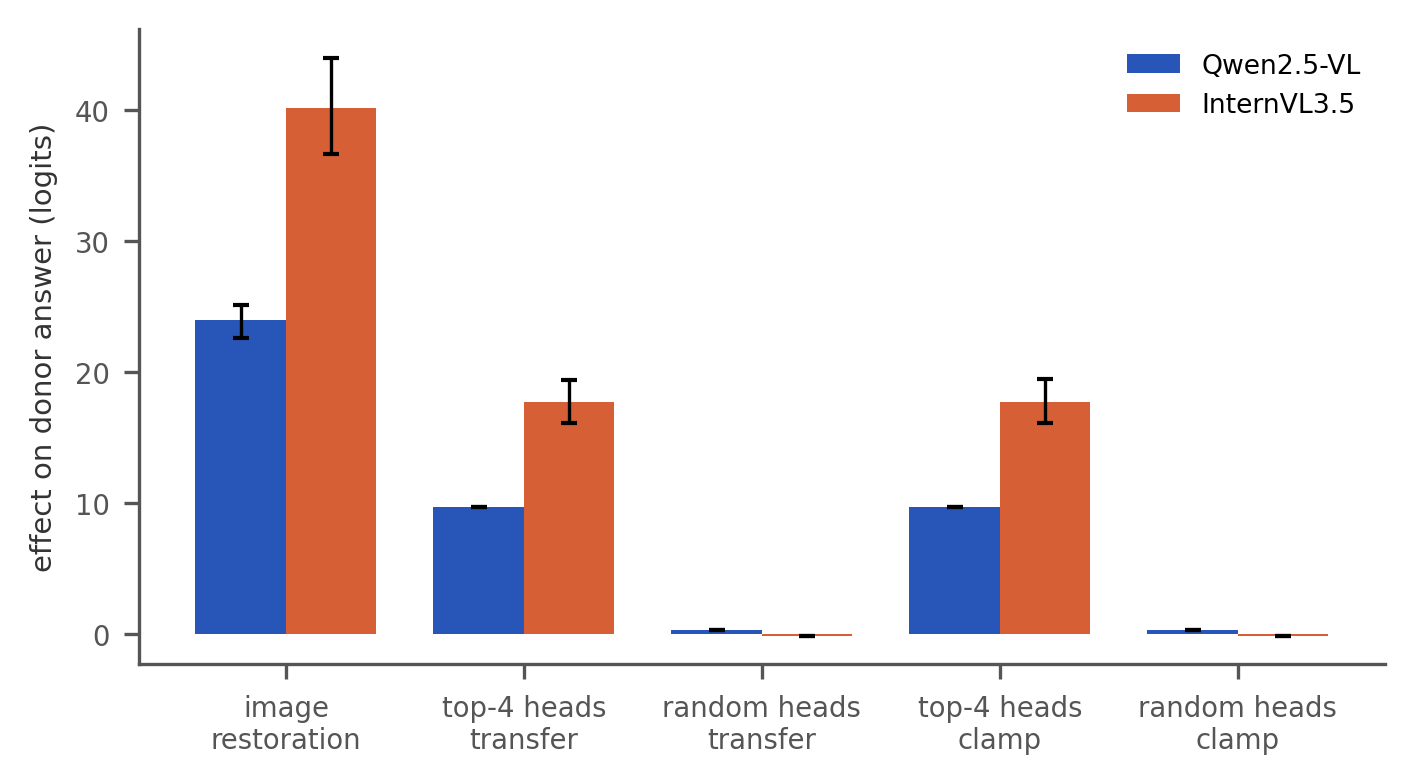
\includegraphics[width=0.94\linewidth]{assets/ext_e20.png}\par
\vspace{0.10cm}
\raggedright
\lesson{\textbf{What we learned.} The early image states carry essentially the whole answer, and the four frozen heads carry a large, selective share of it: copying them transfers it and clamping them blocks it.}\par
\vspace{0.12cm}
{\fontsize{7.2}{8.7}\selectfont\textbf{How it differs from Core-7.} Core-7 tests image tokens (M6) and heads (M3) separately, and chose its heads on same-image contrasts. S1 changes only the image and tests in one run whether those heads carry its effect (copy) and are needed for it (clamp).\par}
\end{columns}
\end{frame}

\begin{frame}{S2: Can a wrong printed symbol be repaired?}
\begin{columns}[T,onlytextwidth]
\column{0.47\textwidth}
\raggedright\fontsize{7.3}{8.6}\selectfont
\textbf{Question}\par \emph{The model sometimes ``knows'' the answer word but prints the wrong letter. Can patching fix the letter?}

\vspace{0.10cm}
\textbf{What we did}\par
\textbf{1. Errors:} from saved records, take prompts where the lens favours the right word (e.g.\ ``yellow'', option C) but a wrong letter is printed.\par
\textbf{2. Donor:} the same image with the options reordered, answered correctly (``yellow'' is now option A).\par
\textbf{3. Patch:} V1 copies only the donor's state over ``yellow''. V2 copies all four option words onto the same words in the recipient, keeping its letters. A real repair prints C (its own letter), not A (the donor's).

\vspace{0.10cm}
\textbf{Results}\par
\textbf{V1} made the errors worse at every layer tried. \textbf{V2} (layer 20) pushed 35 new errors (from scenes not used to choose the layer) toward the right letter (+0.19 logits on average), but fixed only about 1 in 8 (12.9\%): the push is small, so only nearly-right errors flip. Correct cases were almost never harmed (2 of 72).\par
\textbf{InternVL:} no layer gave a valid repair. \textbf{LLaVA:} its readout matched the truth in only 72\% of scenes, too weak to find such errors, so no repair was tested.
\column{0.50\textwidth}
\centering
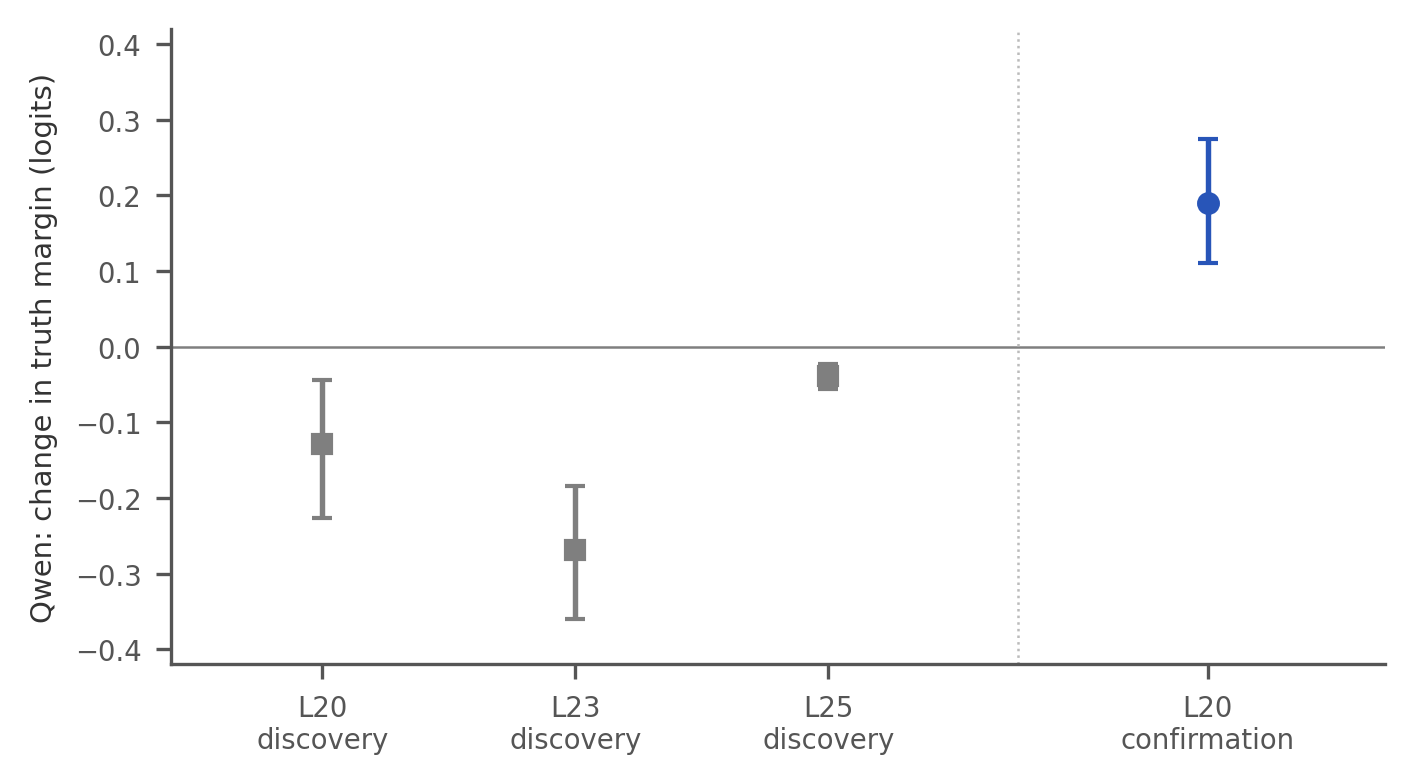
\includegraphics[width=\linewidth]{assets/ext_e22.png}\par
\vspace{0.10cm}
\raggedright
\lesson{\textbf{What we learned.} Copying the right answer word alone does not fix the letter. Copying all four options helps a little, which suggests the model represents the options together. The repair is small: most errors stay wrong.}\par
\vspace{0.12cm}
{\fontsize{7.2}{8.7}\selectfont\textbf{How it differs from Core-7.} Core-7 only patches pairs the model answers correctly and asks where the answer travels. S2 starts from the model's own errors and asks whether patching can repair them.\par}
\end{columns}
\end{frame}

\begin{frame}{S3: Do the heads route to specific image regions?}
\begin{columns}[T,onlytextwidth]
\column{0.47\textwidth}
\raggedright\fontsize{7.3}{8.8}\selectfont
\textbf{Question}\par \emph{When the model answers, do the selected heads look at the object the question asks about, or at the objects that match the answer options?}

\vspace{0.10cm}
\textbf{What we did}\par
Core-7 swapped all image tokens at once (M6), so it could not say \emph{which part} of the image matters. S3 tests specific regions.\par
\textbf{Regions.} In CLEVR scenes we mark two regions: the \emph{question object} (the object the question names) and the \emph{option objects} (the objects whose colours appear among the options).\par
\textbf{Block.} We stop the frozen heads from looking at one region from the answer token, and measure how much the correct answer's lead drops.\par
\textbf{Control.} We also block a patch of plain background with the same number of image tokens. Only harm \emph{beyond} this patch counts.\par
\textbf{Layer.} On a first set of scenes we tried several image layers and kept the one where erasing the region hurt most compared with the control (Qwen 8, InternVL 5, LLaVA 4). We then tested once on new scenes.
\column{0.50\textwidth}
\centering
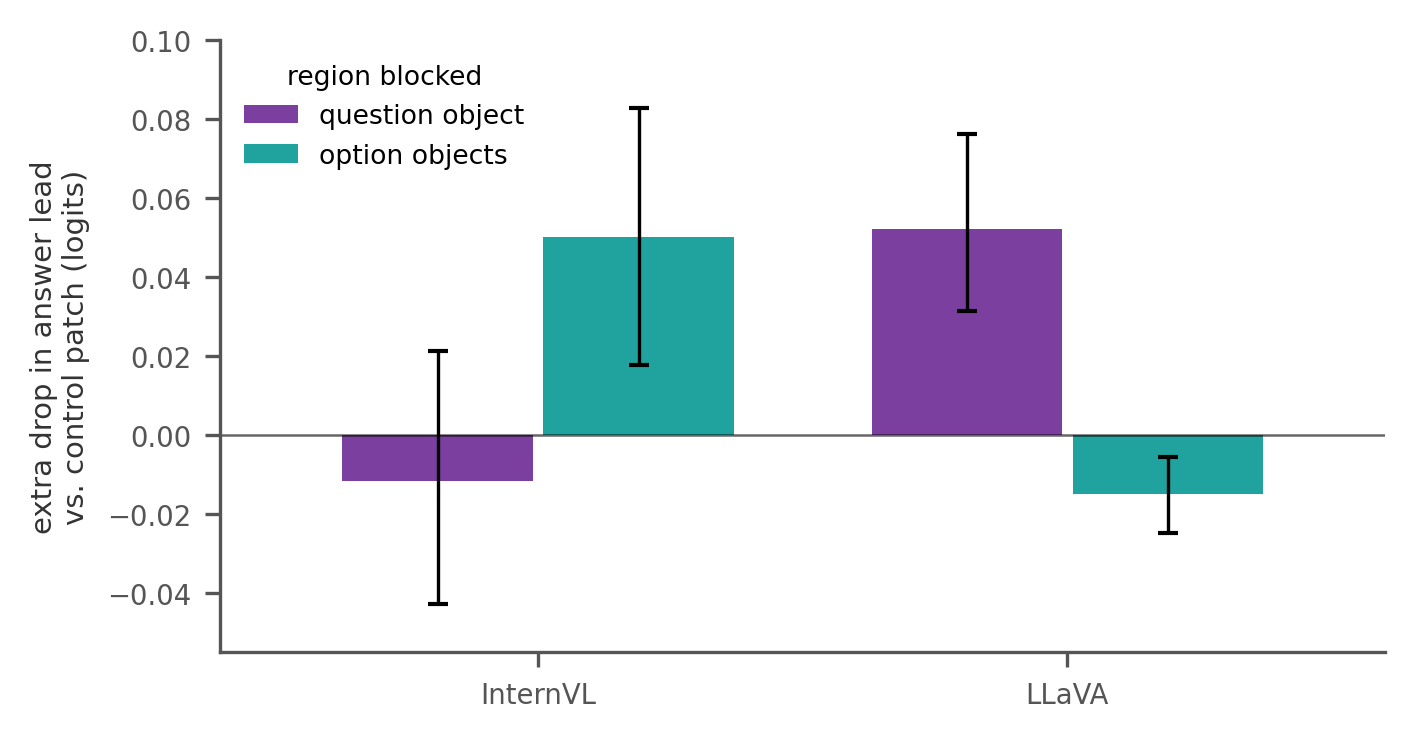
\includegraphics[width=0.80\linewidth]{assets/ext_e23.png}\par
\vspace{0.08cm}
\raggedright
\lesson{\textbf{Results and what we learned.} A region counts as used if, on the new scenes, blocking it hurts more than the background patch (95\% interval above zero).\par
\vspace{2pt}
\textbf{Qwen:} neither region beat the background patch, even when blocking 16 heads.\par
\textbf{InternVL:} blocking the option objects hurt more (+0.05 logits); the question object did not.\par
\textbf{LLaVA:} the reverse: the question object hurt more (+0.05); the option objects did not.\par
\vspace{2pt}
The heads do read from specific objects, but \emph{which} ones differs by model and the effects are small: there is no shared spatial route.}
\end{columns}
\end{frame}

\begin{frame}{S4: With image answer options, content or symbol?}
\begin{columns}[T,onlytextwidth]
\column{0.48\textwidth}
\raggedright\fontsize{7.3}{8.8}\selectfont
\textbf{Question}\par \emph{When the answer options are pictures instead of words, do the frozen heads carry \emph{what} the answer is, or just \emph{which letter} the donor printed?}

\vspace{0.08cm}
\centering
\resizebox{0.72\linewidth}{!}{%
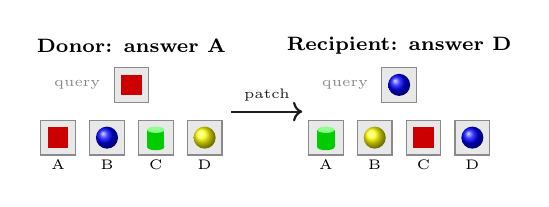
\begin{tikzpicture}[font=\scriptsize]
% donor collage
\node[font=\scriptsize\bfseries] at (0.93,1.12) {Donor: answer A};
\panel{0.93}{0.62}\objcube{red}{0.93}{0.62}
\node[font=\tiny,text=Slate,anchor=east] at (0.66,0.62) {query};
\foreach \x/\l in {0/A,0.62/B,1.24/C,1.86/D}{\panel{\x}{-0.05}\node[font=\tiny] at (\x,-0.40) {\l};}
\objcube{red}{0}{-0.05}\objball{blue}{0.62}{-0.05}\objcyl{green}{1.24}{-0.05}\objball{yellow}{1.86}{-0.05}
% recipient collage
\node[font=\scriptsize\bfseries] at (4.33,1.12) {Recipient: answer D};
\panel{4.33}{0.62}\objball{blue}{4.33}{0.62}
\node[font=\tiny,text=Slate,anchor=east] at (4.06,0.62) {query};
\foreach \x/\l in {3.4/A,4.02/B,4.64/C,5.26/D}{\panel{\x}{-0.05}\node[font=\tiny] at (\x,-0.40) {\l};}
\objcyl{green}{3.4}{-0.05}\objball{yellow}{4.02}{-0.05}\objcube{red}{4.64}{-0.05}\objball{blue}{5.26}{-0.05}
\draw[->,thick,Navy] (2.2,0.28) -- node[above,font=\tiny,align=center] {patch} (3.1,0.28);
\end{tikzpicture}}\par
{\fontsize{6.6}{8}\selectfont Prompt: ``Which option image matches the query image? Respond with only its displayed symbol.''\par}
\raggedright
\vspace{0.08cm}
\textbf{What we did}\par
Unlike Core-7, the options are pictures, and the query copies one of them. Donor and recipient show the same objects in different orders. Two separate patches:\par
\textbf{Panel patch:} copy the donor's hidden states for \emph{one} picture (its query, or the option showing its answer) into the matching recipient picture, at layer 0; everything else stays.\par
\textbf{Head patch:} copy only the frozen top-4 heads' outputs at the answer token.\par
If the \emph{content} moves, the recipient answers C; if the \emph{symbol} moves, A.
\column{0.49\textwidth}
\centering
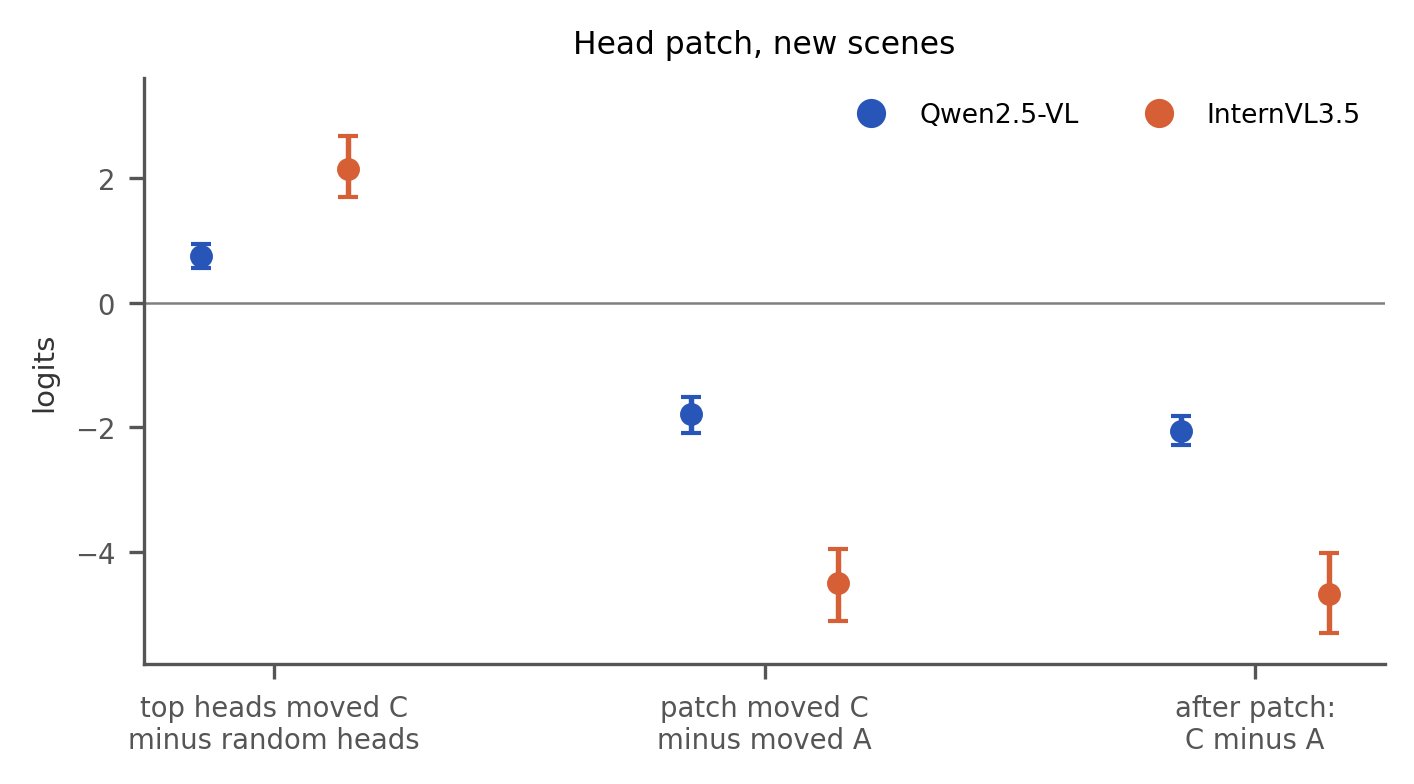
\includegraphics[width=0.76\linewidth]{assets/ext_e24.png}\par
\vspace{0.08cm}
\raggedright
\lesson{\textbf{Results and what we learned.} All numbers compare the model's scores (logits) for \textbf{C}, the letter of the donor's object in the recipient, and \textbf{A}, the donor's own letter.\par
\vspace{2pt}
\textbf{Panel patch:} C's score rose 1.60 more than A's (Qwen, first scenes): the picture content transfers.\par
\textbf{Head patch:} copying the top-4 heads raises C's lead more than copying random heads (+0.75 Qwen, +2.15 InternVL), so the heads matter. But A rises even more: C's gain minus A's gain is $-1.79$ and $-4.49$, and after the patch A is still ahead of C by 2.05 and 4.66.\par
\vspace{2pt}
Early picture tokens carry the object, but the answer heads carry the \emph{letter}. LLaVA: still running.}
\end{columns}
\end{frame}


%======================================================================
\sectionslide{Conclusion}

\begin{frame}{Conclusions}
\begin{columns}[T,onlytextwidth]
\column{0.48\textwidth}
\raggedright
{\footnotesize\bfseries HOLDS ACROSS MODELS\par}
\vspace{0.14cm}
\methoditem{1}{A staged route to the answer}{Image tokens carry the answer early (layer 0), option and question tokens carry it in the middle, and a late attention layer writes it to the answer token at about 65--85\% depth. This holds in all four models and on IconQA.}
\methoditem{2}{A few answer-mover heads}{Small frozen head sets beat the best 5\% of random head sets in every model. In S1, copying only the top-4 heads moves the answer by +9.7 (Qwen) and +17.7 logits (InternVL), against about 0 for random heads.}
\methoditem{3}{The label is decided late}{The label becomes readable at about 70--90\% depth under both lenses. The Tuned Lens shows the requested alphabet is already chosen in the middle layers.}
\column{0.02\textwidth}
\centering
{\color{Gold}\rule{0.4pt}{5.4cm}}
\column{0.46\textwidth}
\raggedright
{\footnotesize\bfseries DEPENDS ON THE MODEL, OR FAILS\par}
\vspace{0.14cm}
\methoditem{4}{Model-specific details}{Transfer layers, the order of content and position, InternVL's head sparsity and the image region the heads read (InternVL: option objects; LLaVA: question object; Qwen: neither).}
\methoditem{5}{Binding content to a symbol}{Repair is small: copying all four options fixes only 12.9\% of Qwen's errors. With picture options the heads copy the donor's \emph{letter}, not its object (after patching, C minus A: $-2.05$ Qwen, $-4.66$ InternVL).}
\methoditem{6}{Transfer to IconQA}{Almost every CLEVR finding transfers, including the CLEVR-chosen heads; only the content/position order does not.}
\end{columns}
\vspace{0.06cm}
\lesson{\textbf{Overall.} VLMs answer MCQs through one shared set of causally useful sites, from image tokens to option tokens to a few late heads that write the symbol, but how the visual content gets bound to the printed letter is still open.}\par
\end{frame}

\begin{frame}{Limitations}
\begin{columns}[T,onlytextwidth]
\column{0.48\textwidth}
\raggedright
\methoditem{Data}{One synthetic dataset}{Most causal work uses CLEVR. The IconQA check covers one edited, class-imbalanced task template (32 confirmation pairs per model), so findings may not carry over to natural images or expert questions.}
\methoditem{Pairs}{Correct-only pairs}{Each model is patched only on pairs it answers correctly on both sides, which can bias the results towards easy cases.}
\methoditem{Models}{Shared backbones}{Qwen, InternVL and LLaVA all use Qwen-lineage language models. PaliGemma2 adds a Gemma backbone only as an exploratory run (54.4\% accuracy, 76/61 pairs), so a shared route is not universality.}
\column{0.48\textwidth}
\raggedright
\methoditem{Claims}{Useful sites, not a circuit}{Patched sites are causally useful for the tested contrast; they are not a complete or minimal circuit.}
\methoditem{Readouts}{Lenses measure readability}{Logit Lens and Tuned Lens show when information is readable, not that the model uses it. Our Tuned Lens is likely under-trained.}
\methoditem{Compute}{Long, shared runs}{Full Core-7 took 5.5 (Qwen) to 34 hours (LLaVA) per model on shared mixed-GPU clusters, which limited how many models and studies we could run.}
\end{columns}
\end{frame}

\begin{frame}{Limitations in Stretch Goals}
\vspace{0.2cm}
\footnotesize
\renewcommand{\arraystretch}{1.45}
\begin{tabularx}{\textwidth}{@{}>{\bfseries\raggedright\arraybackslash}p{2.6cm}>{\raggedright\arraybackslash}X>{\raggedright\arraybackslash}X>{\raggedright\arraybackslash}X>{\raggedright\arraybackslash}X@{}}
\toprule
 & Qwen & InternVL & LLaVA & PaliGemma2 \\
\midrule
S1 image restoration & strong positive & strong positive & not run in time & not run \\
S2 error repair & all-option narrow positive & no layer passed discovery & readout too unreliable & not run \\
S3 spatial routing & no selective edge & option-region sensitivity & question-region sensitivity & not run \\
S4 visual options & symbol-copy pattern & symbol-copy pattern & running & not run \\
IconQA reduced Core-7 & complete; order unstable & complete & complete & changed prompt \\
\bottomrule
\end{tabularx}
\end{frame}

\begin{frame}{Next Steps}
\begin{columns}[T,onlytextwidth]
\column{0.48\textwidth}
\raggedright
\methoditem{1}{Complete the LLaVA row}{Run LLaVA S1 (image restoration) and finish S4 (picture options) so all three main models have every stretch study.}
\methoditem{2}{A non-Qwen backbone}{Run PaliGemma2 with an admission-passing setup, then S1--S4, to test whether the route holds beyond Qwen-lineage models.}
\column{0.48\textwidth}
\raggedright
\methoditem{3}{Beyond one template}{Extend to other IconQA tasks, natural images and native (unedited) counterfactual pairs.}
\methoditem{4}{From sites to a circuit}{Use path patching to connect image tokens, option tokens and the answer-mover heads into one tested route, and train the Tuned Lens longer.}
\end{columns}
\end{frame}

%======================================================================
\sectionslide{Appendix}

\begin{frame}{Dataset scale}
\begin{columns}[T,onlytextwidth]
\column{0.63\textwidth}
\scriptsize
\renewcommand{\arraystretch}{1.12}
\begin{tabularx}{\linewidth}{@{}>{\bfseries}p{1.55cm}>{\raggedright\arraybackslash}X>{\raggedright\arraybackslash}X@{}}
\toprule
Unit & CLEVR-MCQ-4 & IconQA subset \\
\midrule
Items & \textbf{1,252}: 676 single images + 288 pairs $\times$ 2 & \textbf{272}: 136 pairs $\times$ 2, plus 136 same-answer control images \\
Prompt variants & \textbf{17,328} $=$ 1,252 $\times$ 12 $+$ 576 $\times$ 4 & \textbf{4,352} $=$ 272 $\times$ 12 $+$ 272 $\times$ 4 \\
Directed contrasts & \textbf{14,400} $=$ 288 pairs $\times$ 50 & \textbf{2,448} $=$ 136 pairs $\times$ 18 \\
Reasoning families & 9 & 1 (marble probability) \\
\bottomrule
\end{tabularx}

\vspace{0.14cm}
\textbf{Prompt variants.} Every item has 12 variants: 4 option orders $\times$ 3 label sets (A/B/C/D, 1/2/3/4, Q/Z/R/X). Each pair image adds 4 distractor-identity variants for the specificity control.

\vspace{0.08cm}
\textbf{Directed contrasts.} A contrast is one donor $\rightarrow$ recipient patch; each direction counts separately. CLEVR uses the 288 discovery $+$ confirmation pairs, each giving 50: 16 position, 8 content, 8 content $+$ position, 16 distractor-identity and 2 random. IconQA keeps a reduced 18 per pair: 4 of each of the four types and 2 random.

\column{0.33\textwidth}
\scriptsize
\colorbox{Mist}{\parbox{0.94\linewidth}{%
\textbf{Side note: specificity controls}\par\vspace{0.04cm}
Comparisons that should \emph{not} carry the answer effect. A real effect should be larger for the matched counterfactual donor than for these.\par\vspace{0.10cm}
\textbf{Distractor-identity control}\par
Reorder the wrong options; the image and correct answer stay fixed.\par
\emph{Does the effect depend on which incorrect answers are present?}\par\vspace{0.10cm}
\textbf{Random patching control}\par
Copy the activation from a different, unrelated scene.\par
\emph{Is the patch carrying the relevant fact, or merely disturbing the model?}}}
\end{columns}
\end{frame}

\end{document}
